\documentclass[12pt,a4paper]{report}

\usepackage{styles/dolgozat}

\usepackage{listings}
\usepackage{styles/cpp}
\usepackage{styles/python}

\usepackage{hyperref}
\usepackage{url}

\begin{document}

\pagestyle{empty} %a címlapon ne legyen semmi=empty, azaz nincs fejléc és lábléc

% A Miskolci Egyetem címere
{\large
\begin{center}
\vglue 1truecm
\textbf{\huge\textsc{Szakdolgozat}}\\
\vglue 1truecm

\includegraphics[width=4.8truecm, height=4truecm]{images/me_logo.png}\\
\textbf{\textsc{Miskolci Egyetem}}
\end{center}}

\vglue 1.5truecm %függõleges helykihagyás

% A szakdolgozat címe, akár több sorban is
{\LARGE
\begin{center}
\textbf{A szakdolgozat címe}
\end{center}}

\vspace*{2.5truecm}
% A hallgató neve, évfolyam, szak(ok), a konzulens(ek) neve
{\large
\begin{center}
\begin{tabular}{c}
\textbf{Készítette:}\\
Szakdolgozó Neve\\
Programtervező informatikus
\end{tabular}
\end{center}
\begin{center}
\begin{tabular}{c}
\textbf{Témavezető:}\\
Piller Imre
\end{tabular}
\end{center}}
\vfill
% Keltezés: Hely, év
{\large
\begin{center}
\textbf{\textsc{Miskolc, 2020}}
\end{center}}

\newpage


\newpage

\pagestyle{empty}

%Feladatkiiras
\begin{flushleft}
\textsc{\bfseries Miskolci Egyetem}\\
Gépészmérnöki és Informatikai Kar\\
Alkalmazott Matematikai Intézeti Tanszék\hspace*{4cm}\hfil \textbf{Szám:}
\end{flushleft}
\vskip 0.5cm
\begin{center}
\large\textsc{\bfseries Szakdolgozat Feladat}
\end{center}
\vskip 0.5cm
Gyulai Márk (NV4AO2) programtervező informatikus jelölt részére.\newline

\noindent\textbf{A szakdolgozat tárgyköre:} kulcsszavak, hasonlók\newline

\noindent\textbf{A szakdolgozat címe:} A dolgozat címe\newline

\noindent\textbf{A feladat részletezése:}

\medskip

\emph{Ide kell a feladatkiírásban szereplő szöveget betenni.}

\medskip

\emph{(Kisebb tagolás lehet benne, hogy jól nézzen ki.)}

\vfill

\noindent\textbf{Témavezető:} Dr. Nagy Noémi (egyetemi adjunktus)

\medskip

\noindent\textbf{Konzulens:} Piller Imre (egyetemi tanársegéd) \newline

% \noindent\textbf{Konzulens(ek):} (akkor kötelezõ, ha a témavezetõ nem valamelyik matematikai tanszékrõl való; de persze lehet egyébként is)\newline

\noindent\textbf{A feladat kiadásának ideje:}\newline

%\noindent\textbf{A feladat beadásának határideje:}

\vskip 2cm

\hbox to \hsize{\hfil{\hbox to 6cm {\dotfill}\hbox to 1cm{}}}

\hbox to \hsize{\hfil\hbox to 3cm {szakfelelős}\hbox to 2cm{}}

\newpage

\vspace*{1cm}  
\begin{center}
\large\textsc{\bfseries Eredetiségi Nyilatkozat}
\end{center}
\vspace*{2cm}  

Alulírott \textbf{Gyulai Márk}; Neptun-kód: \texttt{NV4AO2} a Miskolci Egyetem Gépészmérnöki és Informatikai Karának végzős Programtervező informatikus szakos hallgatója ezennel büntetőjogi és fegyelmi felelősségem tudatában nyilatkozom és aláírásommal igazolom, hogy \textit{Numerikus számítások hatékonyságának vizsgálata Python környezetben}
című szakdolgozatom saját, önálló munkám; az abban hivatkozott szakirodalom
felhasználása a forráskezelés szabályai szerint történt.\\

Tudomásul veszem, hogy szakdolgozat esetén plágiumnak számít:
\begin{itemize}
\item szószerinti idézet közlése idézőjel és hivatkozás megjelölése nélkül;
\item tartalmi idézet hivatkozás megjelölése nélkül;
\item más publikált gondolatainak saját gondolatként való feltüntetése.
\end{itemize}

Alulírott kijelentem, hogy a plágium fogalmát megismertem, és tudomásul veszem, hogy
plágium esetén szakdolgozatom visszautasításra kerül.

\vspace*{3cm}

\noindent Miskolc, \hbox to 2cm{\dotfill} .év \hbox to 2cm{\dotfill} .hó \hbox to 2cm{\dotfill} .nap

\vspace*{3cm}

\hspace*{8cm}\begin{tabular}{c}
\hbox to 6cm{\dotfill}\\
Hallgató
\end{tabular}



\newpage

\noindent 1.

\begin{tabular}{cl}
&szükséges (módosítás külön lapon) \\
A szakdolgozat feladat módosítása& \\
& nem szükséges\\
&\\
\hbox to 4cm{\dotfill}&\multicolumn{1}{c}{\hbox to 5cm{\dotfill}}\\
dátum& \multicolumn{1}{c}{témavezető(k)}
\end{tabular}
\vskip1.5mm

\noindent 2. A feladat kidolgozását ellenőriztem:

\vskip1.5mm

\begin{tabular}{l@{\hspace*{4cm}}l}
témavezető (dátum, aláírás):& konzulens (dátum, aláírás):\\
\dotfill&\dotfill\\
\dotfill&\dotfill\\
\dotfill&\dotfill
\end{tabular}

\vskip1.5mm

\noindent 3. A szakdolgozat beadható:

\vskip1.5mm

\begin{tabular}{@{\hspace*{1.3cm}}c@{\hspace*{2.1cm}}c}
\hbox to 4cm{\dotfill}&\multicolumn{1}{c}{\hbox to 5cm{\dotfill}}\\
dátum& \multicolumn{1}{c}{témavezető(k)}
\end{tabular}

\vskip1.5mm

\noindent 4.
\begin{tabular}[t]{@{}l@{\hspace*{1mm}}l@{\hspace*{1mm}}l@{}}
A szakdolgozat& \hbox to 3.5cm{\dotfill} &szövegoldalt\\
              & \hbox to 3.5cm{\dotfill} &program protokollt (listát, felhasználói leírást)\\
              &\hbox to 3.5cm{\dotfill}   &elektronikus adathordozót (részletezve)\\
              &\hbox to 3.5cm{\dotfill} & \\
              &\hbox to 3.5cm{\dotfill} &egyéb mellékletet (részletezve)\\
              &\hbox to 3.5cm{\dotfill} &\\
\end{tabular}
\newline tartalmaz.

\vskip1.5mm

\begin{tabular}{@{\hspace*{1.3cm}}c@{\hspace*{2.1cm}}c}
\hbox to 4cm{\dotfill}&\multicolumn{1}{c}{\hbox to 5cm{\dotfill}}\\
dátum& \multicolumn{1}{c}{témavezető(k)}
\end{tabular}

\noindent 5.

\begin{tabular}{ll}
&bocsátható\\
A szakdolgozat bírálatra& \\
& nem bocsátható\\
\end{tabular}

\vskip1.5mm

\noindent A bíráló neve: \hbox to 8cm{\dotfill}

\vskip4mm

\begin{tabular}{@{\hspace*{1.3cm}}c@{\hspace*{2.1cm}}c}
\hbox to 4cm{\dotfill}&\multicolumn{1}{c}{\hbox to 5cm{\dotfill}}\\
dátum& \multicolumn{1}{c}{szakfelelős}
\end{tabular}

\noindent 6.
\begin{tabular}[t]{@{}l@{\hspace*{1mm}}l@{\hspace*{1mm}}l@{}}
A szakdolgozat osztályzata& &\\
&a témavezető javaslata:& \hbox to 3cm{\dotfill}\\
&a bíráló javaslata:& \hbox to 3cm{\dotfill}\\
&a szakdolgozat végleges eredménye:& \hbox to 3cm{\dotfill}
\end{tabular}

\vspace*{4mm}

\noindent Miskolc, \hbox to 4.5cm{\dotfill} \hspace*{2.5cm}
\begin{tabular}[t]{cc}
\hbox to 6cm{\dotfill}\\
a Záróvizsga Bizottság Elnöke
\end{tabular}


\cleardoublepage
\pagenumbering{gobble}
\tableofcontents
\cleardoublepage
\pagenumbering{arabic}

\newpage

\pagestyle{fancy}

\Chapter{Bevezetés}


\Chapter{Python}

\section{Bevezető}\label{bevezetux151}

    Ebben a rövid fejezetben szeretném a kedves Olvasónak reprezentálni
miről is szól a szakdolgozat, mi a témája, mit használtam fel benne,
mire is van szükség ha ki szeretné próbálni a benne található kódokat.
Vágjunk is bele! Először is a téma: a szakdolgozat témája a tanult
numerikus számítási ejárások Python környezetben való bemutatása. Ilyen
numerikus problémák például a mátrix transzponálás mátrix felbontások
(LU, Cholesky), lineáris egyenetrendszerek megoldása, interpolációk
felírása, vagy a numerikus deriválás és integrálás. A numerikus
eljárások mindig az egzakt megoldáshoz közelítő értéket fognak megadni.
Ilyen problémákra már sokféle szoftvert fejlesztettek ki. Például a
Matlab, de akár az R környezetet is használhatjuk ilyen célokra. De
akkor miért Python? - teheti fel a kérdést a kedves Olvasó. A válaszom
pedig az, hogy a dolgozatomban azt fogom bemutatni, hogy, mint sokminden
máshoz ehhez is tökéletesen megfelel és könnyen használható ez a nyelv.
A következő szakaszban magáról a Python nyelvről fogok írni általánosan,
majd áttekintem a dolgozat fő részeit.

    \subsubsection{Mi is az a Python?}\label{mi-is-az-a-python}

    A Python egy nagyon magas szintű, platform független, általános
programozási nyelv szóval itt nem a kígyófélék egy családjára vagy Monty
Pythonra (bár a nevét a a Monty Python csapatról kapta) kell gondolni.
Egy könnyen elsajátítható programozási nyelv mely jelen pillanatban a 3
legnépszerűbb között van a világon (2020 Február). A nyelv interpretált
és támogatja a objektum orientált, a funkcionális, az imperatív és a
procedurális programozási paradigmákat, valamint a dinamikus típusokat
és dinamikus memóriakezelést (használ \emph{garbage collector}t). A
nyelvet Guido van Rossum holland programozó kezdte el fejleszteni
1989-ben, majd nyilvánosságra hozta 1991-ben. Ez volt a 0.9-es
verziószámú. 1994-ben megjelent az 1.0-ás majd 2000-ben a 2.0-ás verzió
és csak 2008-ban követte a dolgozatban általam is használt Python 3. A a
3-as és a 2-es nem minden esetben kompatibilis egymással és a 2-es
utolsó támogatott verzióinak (2.7.x) a támogatása is megszűnt 2020
januárban. A nyelvet napjainkban már a PSF (\emph{Python Software
Foundation}) fejleszti és kezeli.

    \subsubsection{Felhasználása különböző
területeken}\label{felhasznuxe1luxe1sa-kuxfcluxf6nbuxf6zux151-teruxfcleteken}

    A Python nyelvet sok területen felhasználják, többek között

\begin{itemize}
\item
  Webfejlesztésben,
\item
  Tudományos és numerikus számításoknál,
\item
  Oktatásban,
\item
  Asztali grafikus felhasználói felűletek (GUI) fejlesztésében,
\item
  Szoftverfejlesztésben,
\item
  Üzleti szoftverek fejlesztésében.
\end{itemize}

Látható tehát hogy tényleg sok helyen jól használható ez a nyelv.

    \subsubsection{Mi szükséges a
hozzá?}\label{mi-szuxfcksuxe9ges-a-hozzuxe1}

    Tulajdonképpen csak egy számítógép, a Python interpreter és egy
támogatott operációs rendszer, amit nem lesz nehéz találni hiszen a
nyelv minden ma használt és elterjedt operációs rendszert támogat. Az
interpreter pedig letölthető a python weboldaláról (www.python.org),
illetve egyes operációs rendszerekben alapértelmezés szerint telepítve
van (különböző linux disztribúciók).

    \subsubsection{Milyen problémákkal fog foglalkozni a
dolgozat?}\label{milyen-probluxe9muxe1kkal-fog-foglalkozni-a-dolgozat}

    Ahogy már fent említettem, a dolgozat Python-ban fogja bemutatni a
tanult numerikus problémákat és módszereket, melyekkel egy közelítő
megoldást adhatunk egy-egy problémára. Ilyen prolémák:

\begin{itemize}
\item
  Hibaszámítás: Abszulút és relatív hiba
\item
  Vektor és mátrix műveletek
\item
  Lineáris egyenletrendszerek megoldása
\item
  Interpolációk
\item
  Numerikus deriválás
\item
  Numerikus Integrálás
\item
  Sajátérték és sajátvektor
\end{itemize}

Ezeken belül is az ilyen módszerekkel fogok dolgozni, mint például:

\begin{itemize}
\item
  Gauss módszer
\item
  Gauss-Jordan módszer
\item
  Legkisebb négyzetek módszere
\item
  Lagrange interpolációk
\item
  Spline interpolációk
\item
  Téglalap módszer
\item
  Trapéz módszer
\end{itemize}



\Chapter{Szoftvereszközök numerikus számításokhoz}

\section{Szoftvereszközök numerikus
számításokhoz}\label{szoftvereszkuxf6zuxf6k-numerikus-szuxe1muxedtuxe1sokhoz}

    A numerikus számítások lényege, hogy valamilyen algoritmust végrehajtva
eljutunk a probléma egy közelítő megoldásához és ezt egy számítógépes
program segítségével tesszük. Ez a program lehet egy előre megírt
program csomag része, de akár írhatunk magunk is specifikus problémákra
saját programokat. Ezt megtehetjük akár egy olyan eltejedt általános
programozási nyelven, mint például a \textbf{C} vagy a \textbf{Java,} de
akár használhatunk egy ilyen feladatokra készített nyelvet vagy
programcsomagot is. A különbség a nehézségben és az időben rejlik,
hiszen az egyiket erre találták ki, előre definiálva vannak benne
szükséges függvények, konstansok, míg a másikban alapjaitól fel kell
építeni szinte mindent. Szerencsére jópár, numerikus számításokhoz
használható szoftvercsomag és nyelv létezik, ebben a fejezetben ezekről,
és ezek előnyeiről és hátrányairól fogok írni, illetve a fejezet végén
szó esik majd a \textbf{Python} eszközkészletéről is.

    \subsection{Alapvető elvárások}\label{alapvetux151-elvuxe1ruxe1sok}

    Először is beszéljünk az alapvető elvárásokról, amiket egy ilyen
nyelvvel vagy szoftvercsomaggal szemben felállíthatunk. Kezdjük a
programozhatósággal, fontos, hogy tudjunk benne programokat írni, hogy
speciális feladatokat tudjunk vele megoldani, esetlegesen új módszereket
tudjunk implementálni vagy csak egy módszer optimális implementációját
szeretnénk elkészíteni és ne csak olyan problémákra adjon a
programcsomag megoldást amit előzetesen annak fejlesztői implementáltak.
A programozhatóság ebben a kontextusban elég, ha lekorlátozódik arra,
hogy itt matematikai problémák megoldására tudjunk programokat írni,
ezért nem feltétlenül kell általános nyelvnek lennie, erre jó példa a
\textbf{Matlab}, amit mátrix műveletekhez optimalizáltak vagy az
\textbf{R} ami egy statisztikai programcsomag. Ellenpélda a
\textbf{Python}, mely egy általános célú nyelv de a \texttt{NumPy} és
\texttt{SciPy} csomag segítségével használhatunk numerikus problémák
megoldására.

A programozhatóság mellett fontos még a programozási nyelv milyensége.
Általában matematikusok, kutatók, mérnökök használják ezeket tudományos
vagy mérnöki célokra, illetve diákoknak tanítják a numerikus módszereket
ezekkel a programcsomagokkal. Ők itt csak felhasználók, és nem mindig
várható el a felhasználóktól, hogy a programozás minden szempontjával és
fortélyával tisztában legyenek, így egy viszonylag könnyen tanulható és
használható nyelv az, amire szükség van ilyen célokra, lehetőleg
valamilyen egyszerűen megérthető praradigmára építsen, mint az objektum
orientáltság vagy a procedurális programozás, vagy néha elég lehet az
is, ha csak matematikai formában adjuk meg a megoldandó feladatot. A
programozási nyelvek, melyekről itt majd részletesebb is lesz szó, elég
könnyen tanulhatóak (kivétel talán a \textbf{Fortran} ami egy régi,
nehezebben kezelhető nyelv, illetve a \textbf{Wolfram Matematica} eddig
említettektől teljesen eltérő szimbolikus nyelve). Ellenben a
\textbf{WolframAlpha} képes matematikai formában megadott problémákat is
megoldani.

Fontos még ezeken felül, hogy a programokat fájlokba tudjuk menteni és
ezáltal hordozhatóvá tenni őket, és ez nem csak a programok
forráskódjaira legyen igaz, hanem az eredményekre is. Szükséges az, hogy
el lehessen menteni a kapott eredményeket, adatokat későbbi
felhasználás, publikálás illetve áttanulmányozás érdekében. Az érem
másik oldala legalább annyira hasznos és fontos, be is kell tudni
olvasni az adatokat különböző adastruktúrákból, különböző formátumú
fájlokból, ezért szükséges a népszerűbb adatfájl formátumok támogatása,
mint például a CSV, JSON, XML vagy csak egy sima szöveges (.txt) fájl.

Az adatok mentése mellett a bemutatásuk is fontos lehet hiszen az
emberek nagy része a grafikus ábrákból egyszerűbben letudja olvasni az
adatokat, ezért szükséges, hogy a program csomag valamilyen módon tudjon
ábrákat készíteni. A programokat és módszereket nem csak megírni,
menteni és reprezentálni kell, hanem dokumentálni is azokat ezért
szükséges hogy az adott nyelvnek és csomagnak ezt támogatnia kell. Egy
nagyon jó példa erre a \textbf{Python} amivel használhatjuk a a
\texttt{Jupyter} munkafüzetet melyben a dokumentum cellákból épül fel és
a cellákban egyszerre tudunk programozni és dokumentálni is.

A teljesítmény egy nagyon triviális követelmény, de egy nagyon fontos
tényező is, bár nagyon nagy adatokhoz szükséges egy erős hardver, de
szükséges az is, hogy gyengébb hardveren is futtatható legyen a kód
viszonylag jó futási idővel. Erre a problémára egy megoldás még a cloud
(felhő) amihez egy viszonylag gyors internet kapcsolat elég. Egyszerűen
működik, elküldjük a bemenő adatokat és a programot majd visszakapjuk az
eredményt, bár fontos megjegyezni, hogy ez érzékeny adatok esetén ez nem
lehet megoldás hiszen a szerver üzemeltetői láthatják ezeket.

Egy utolsó, de nem elhanyagolható tényező, a programcsomag és az általa
használt nyelv elterjedsége is, hiszen használhatjuk a lehető
leggyorsabb nyelvet ha a világban rajtunk kívül csak még egy páran
használják, de a világ többi része egy másik elfogadott nyelvet használ,
és így nehéz az általunk használt nyelvvel elhelyezkedni, vagy az
adatainkat és programjainkat megosztani másokkal, hiszen nem fogják
érteni és nem tudják majd futtatni.

    \subsection{Elérhető szoftverek}\label{eluxe9rhetux151-szoftverek}

    A fejezet további részében az alábbi programcsomagokkal fogok
foglalkozni: - Fortran - Maple - Matlab - Python NumPy - GNU R - Wolfram
Alpha és Mathematica

    \subsubsection{Fortran}\label{fortran}

    \begin{figure}
\centering
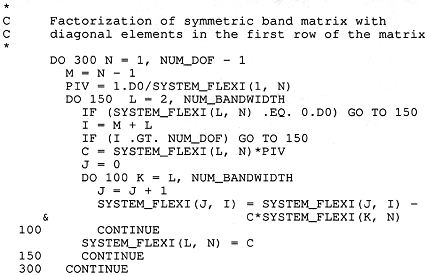
\includegraphics{img/FORTRAN_code_example.png}
\caption{alt text}
\end{figure}

A Fortran egy általános célú programozási nyelv melyet az IBM
fejlesztett ki még az 1950-es években. Napjainkban is használatos és még
napjainkban is fejlesztik. Aránylag nehezen tanulható nyelv ami több
programozási paradigmát is támogat köztük az objektum orientáltságot,
procedurális és generikus programozást is. A Fortran támogatja a fájlba
írást de kimondott különböző fájlformátumú fájlok létrehozását nem, így
ha olyan fájlba szeretnénk az adatainkat menteni, nekünk kell
gondoskodni a formai követelményekről (például: CSV esetén nekünk kell
az elválasztó jelet kiteni az adatok közé).

Weboldal: https://gcc.gnu.org/fortran/, https://wg5-fortran.org/

    \subsubsection{Maple}\label{maple}

    \begin{figure}
\centering

\includegraphics{img/maple_logo.png}
\caption{alt text}
\end{figure}

\begin{figure}
\centering
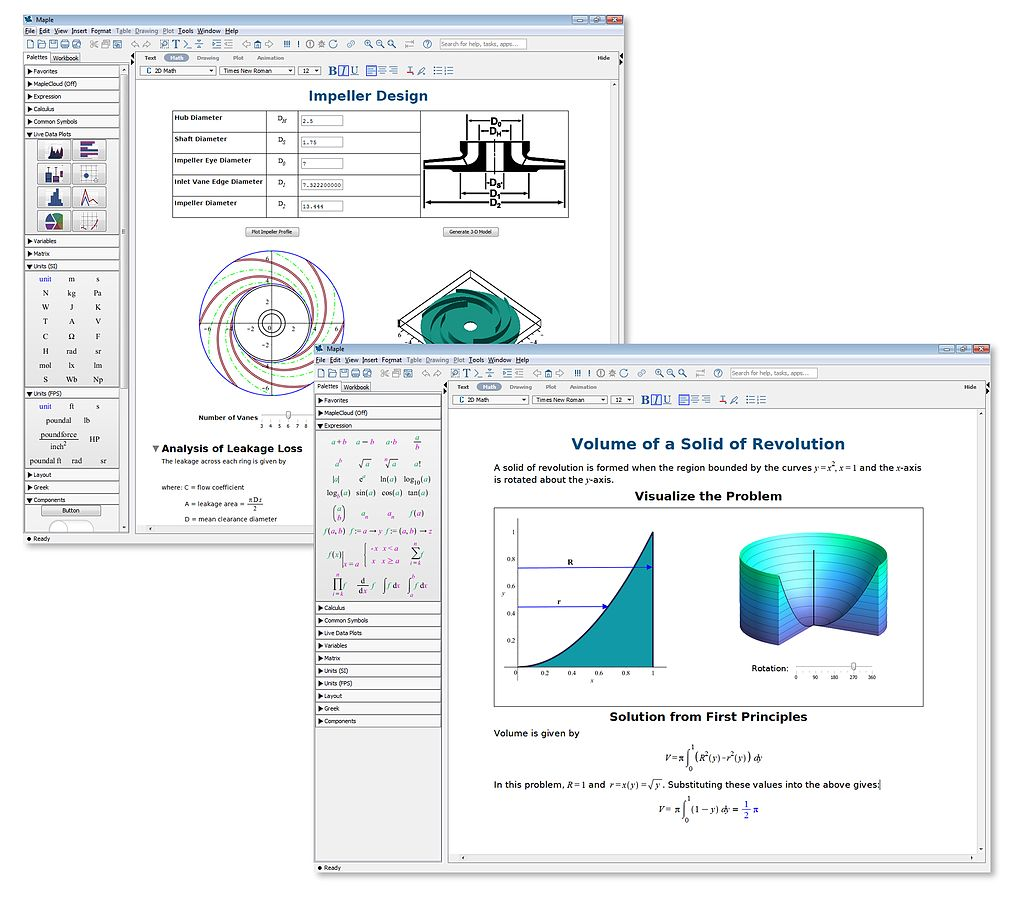
\includegraphics{img/Maple_screenshots.jpg}
\caption{alt text}
\end{figure}

A \textbf{Maple} a Maplesoft által fejlesztett matematikai
szoftvercsomag, mely kombinál egy hatékony matematikai motort, mely a
számításokat végzi és egy könnyen használható felhasználói felületet,
ezáltal a használata egyszerű és gyors is tud lenni. A felhasználói
felület mellett parancssoros módban is képes működni, a saját nyelvét
használva. Scripteket is írhatunk melyet később megtudunk hívni.

A Maple-t mérnöki munkára és emellett rengeteg matematikai területen be
lehet vetni, például numerikus számításoknál, lineáris algebrában,
differenciál egyenleteknél. Nagyszerű az adatok vizualizálásában is. A
Maple nem ingyenes, licenszet kell hozzá vásárolni melynek ára elég
borsos, de itt is elérhető diák kedvezmény, mint a legtöbb ilyen
szoftvercsomag esetében, de 15 napig ingyenesen kipróbálhatja bárki.

Egyik előnye, hogy képes kommunikálni bizonyos szoftverekkel, mint a
Microsoft Excel, néhány CAD szoftver, SQLite adatbázisokkal, és az újabb
Matlab verziókkal is, ezzel könnyítve a munkát. Képes az ismertebb
adattárolásra használt fájlokba menteni és betölteni is, mint CSV, XLS.
Elérhető Microsoft Windowsra, Linuxra, és Apple MacOS-re.

Weboldala: https://www.maplesoft.com/

    \subsubsection{MATLAB}\label{matlab}

    \begin{figure}
\centering

\includegraphics{img/Matlab_Logo.png}
\caption{alt text}
\end{figure}

\begin{figure}
\centering
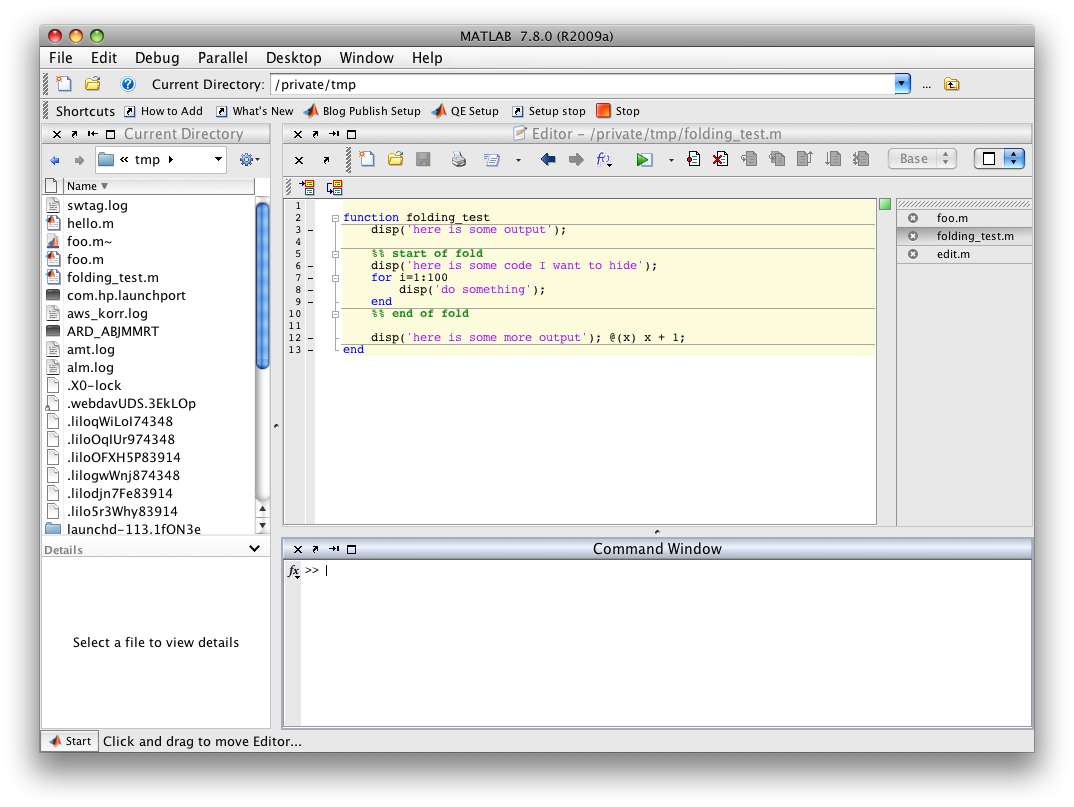
\includegraphics{img/matlab_sreenshots.png}
\caption{alt text}
\end{figure}

A \textbf{Matlab} a MathWorks program csomagja és programozási nyelve is
egyben, egy nagyon elterjedt nyelv a világon és számos helyen használják
különböző célokra mint: numerikus számítások, robotika, adat elemzés,
gépi tanulás, jel feldolgozás, kockázat elemzés, és irányító rendszerek.
Elsődlegesen mátrix műveletekre és numerikus számításokra készült,
ezáltal nagyon jól kezelei a mátrixokat és vektorokat. Szintaktikája a
C-re hasonlít, de vannak eltérések. Képes több szálon dolgozni és
támogatja a procedurális és objektum orientált programozási paradigmákat
is. A Matlab kódokat is menthetjük fájlba, ezáltal tudjuk tárolni,
publikálni (kiterjesztése: .m). Elérhető Microsoft Windows, Linux és
Apple MacOS operációsrendszerű gépekre. A Matlab nem egy ingyenes
szoftver meg kell vásárolni, de van lehetőségünk ingyenesen kipróbálni
illetve van kedvezmény diákok számára. A Matlab is képes importálni és
exportálni az adatokat a leginkább használt fájltípusokból.

MathWorks weboldala: https://www.mathworks.com/

    \subsubsection{Python/NumPy}\label{pythonnumpy}

    \paragraph{Python}\label{python}

\begin{figure}
\centering

\includegraphics{img/python-logo.png}
\caption{alt text}
\end{figure}

\begin{figure}
\centering
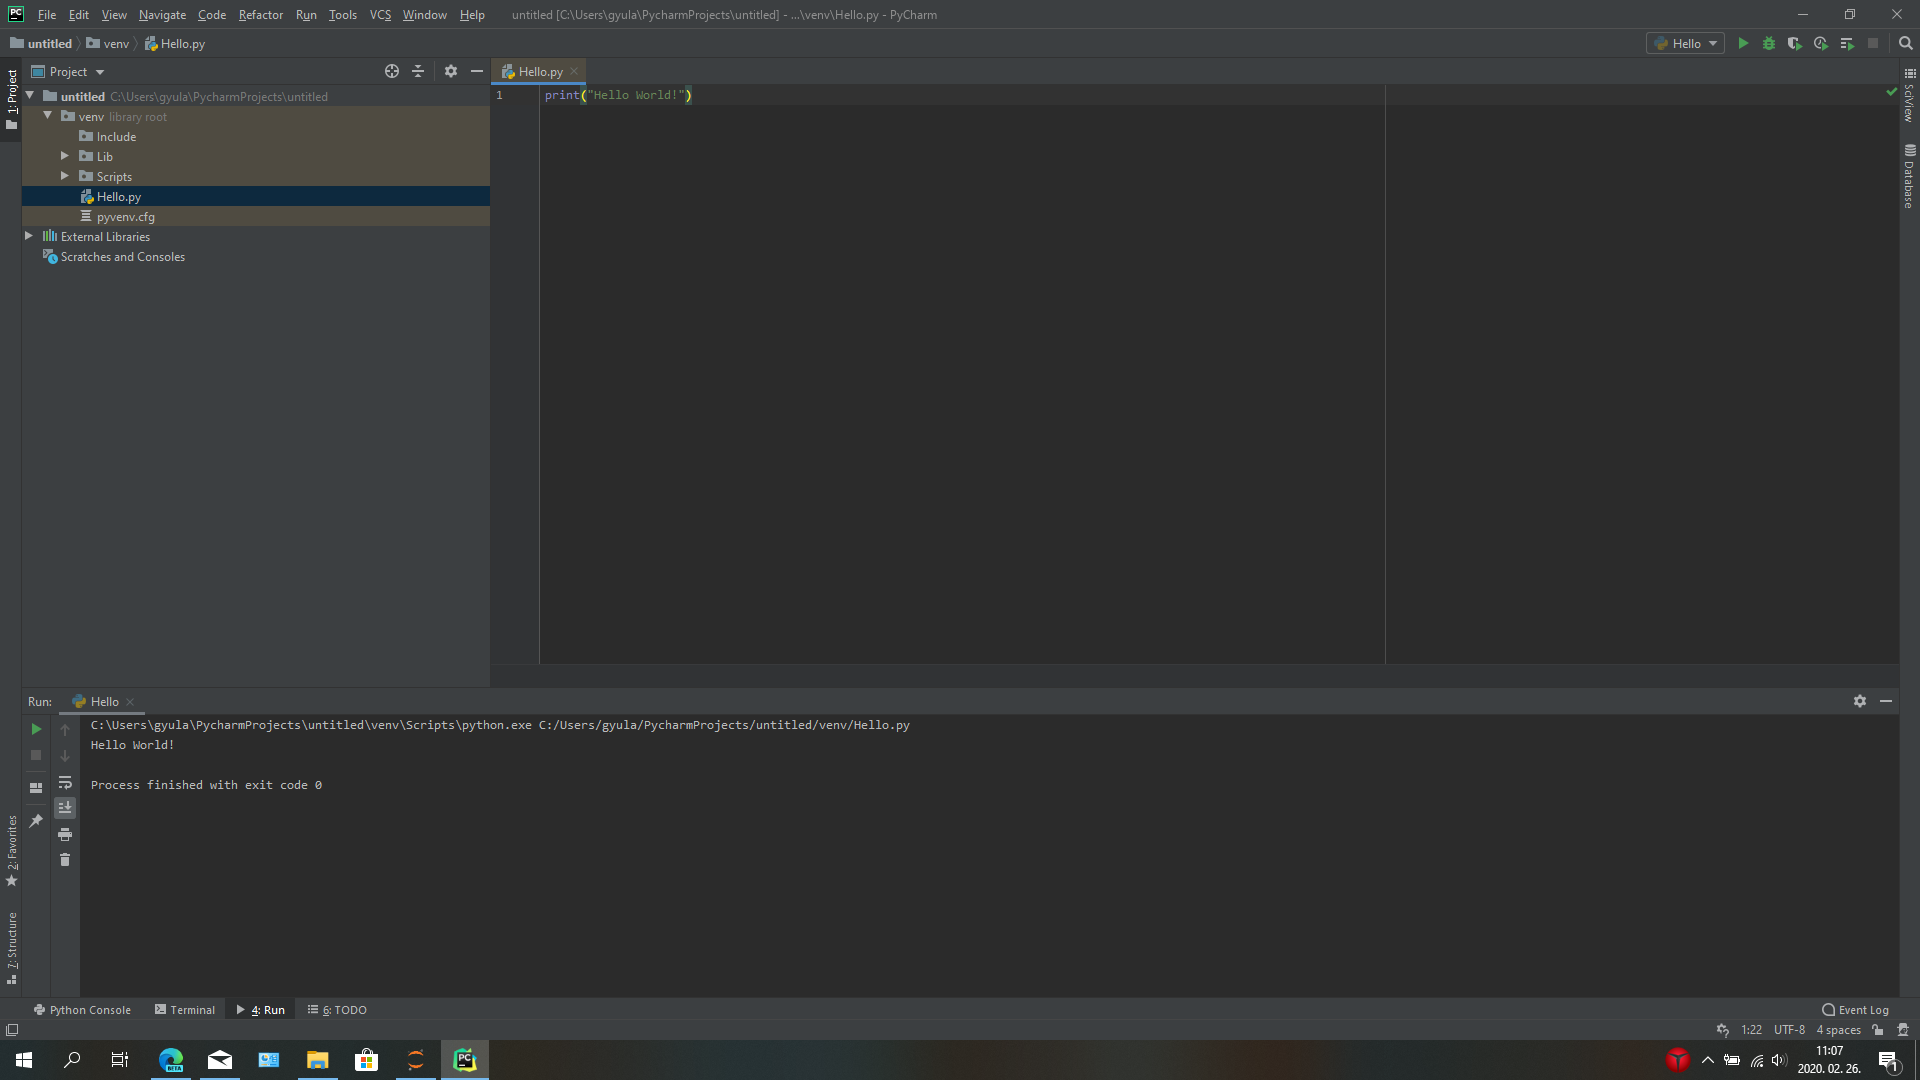
\includegraphics{img/Python_screenshot.png}
\caption{alt text}
\end{figure}

\begin{figure}
\centering
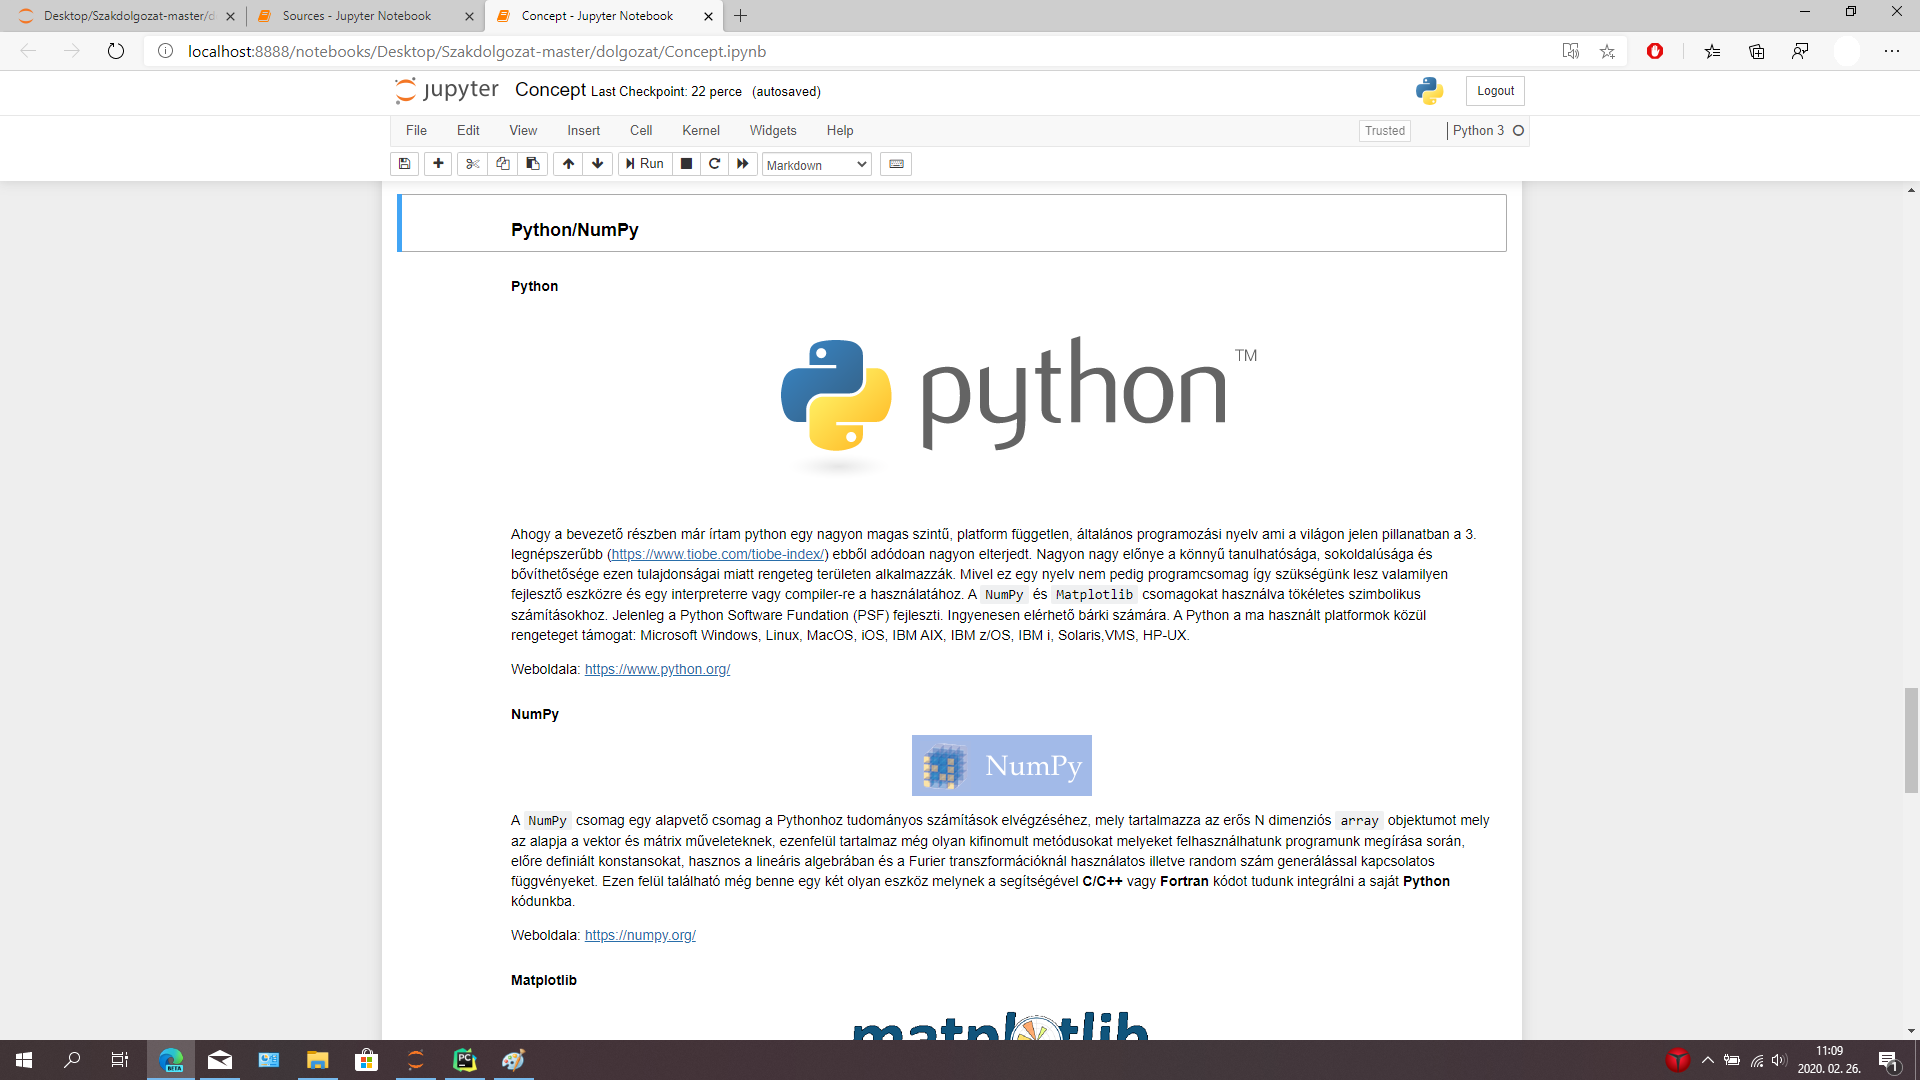
\includegraphics{img/Jupyter_screenshot.png}
\caption{alt text}
\end{figure}

Ahogy a bevezető részben már említettem, a Python egy nagyon magas
szintű, platform független, általános programozási nyelv ami a világon
jelen pillanatban a 3. legnépszerűbb
(https://www.tiobe.com/tiobe-index/) ebből adódóan nagyon elterjedt.
Nagyon nagy előnye a könnyű tanulhatósága és megengedő szintaktikája,
sokoldalúsága és bővíthetősége. Ezen tulajdonságai miatt rengeteg
területen alkalmazzák. Mivel ez egy nyelv, nem pedig programcsomag így
szükségünk lesz valamilyen fejlesztő eszközre és egy interpreterre (vagy
compiler-re) a használatához. A \texttt{NumPy}, \texttt{SymPy},
\texttt{SciPy} és \texttt{Matplotlib} csomagokat használva tökéletes
numerikus és szimbólikus számításokhoz. Jelenleg a Python Software
Fundation (PSF) fejleszti. Ingyenesen elérhető bárki számára. A Python a
ma használt platformok közül rengeteget támogat: Microsoft Windows,
Linux, MacOS, iOS, IBM AIX, IBM z/OS, IBM i, Solaris, VMS, HP-UX, mint
ahogy rengeteg fájltípust is támogat, adat export és adat importálás
szempontjából is.

Weboldala: https://www.python.org/

\paragraph{NumPy}\label{numpy}

A \texttt{NumPy} csomag egy alapvető csomag a Pythonhoz tudományos
számítások elvégzéséhez, mely tartalmazza az erős N dimenziós
\texttt{array} objektumot mely az alapja a vektor és mátrix
műveleteknek, ezenfelül tartalmaz még olyan kifinomult metódusokat
melyeket felhasználhatunk programunk megírása során, előre definiált
konstansokat, hasznos a lineáris algebrában és a Fourier
transzformációknál, illetve véletlenszám generálással kapcsolatos
függvények is elérhetők benne. Ezen felül található még két olyan eszköz
melynek a segítségével \textbf{C/C++} vagy \textbf{Fortran} kódot tudunk
integrálni a saját \textbf{Python} kódunkba.

Weboldala: https://numpy.org/

\paragraph{Matplotlib}\label{matplotlib}

A \texttt{Matplotlib} csomag segítségével tudjuk vizualizálni az
általunk használt adatokat vagy általunk kiszámított adatokat. 2D-s
grafikonokat és ábrákat készíthetünk a segítségével. Az ábrákat tudjuk
menteni is külön fájlba, a Cairo segítségével akár vektorgrafikusan is.

Weboldala: https://matplotlib.org/

    \subsubsection{GNU R}\label{gnu-r}

    \begin{figure}
\centering
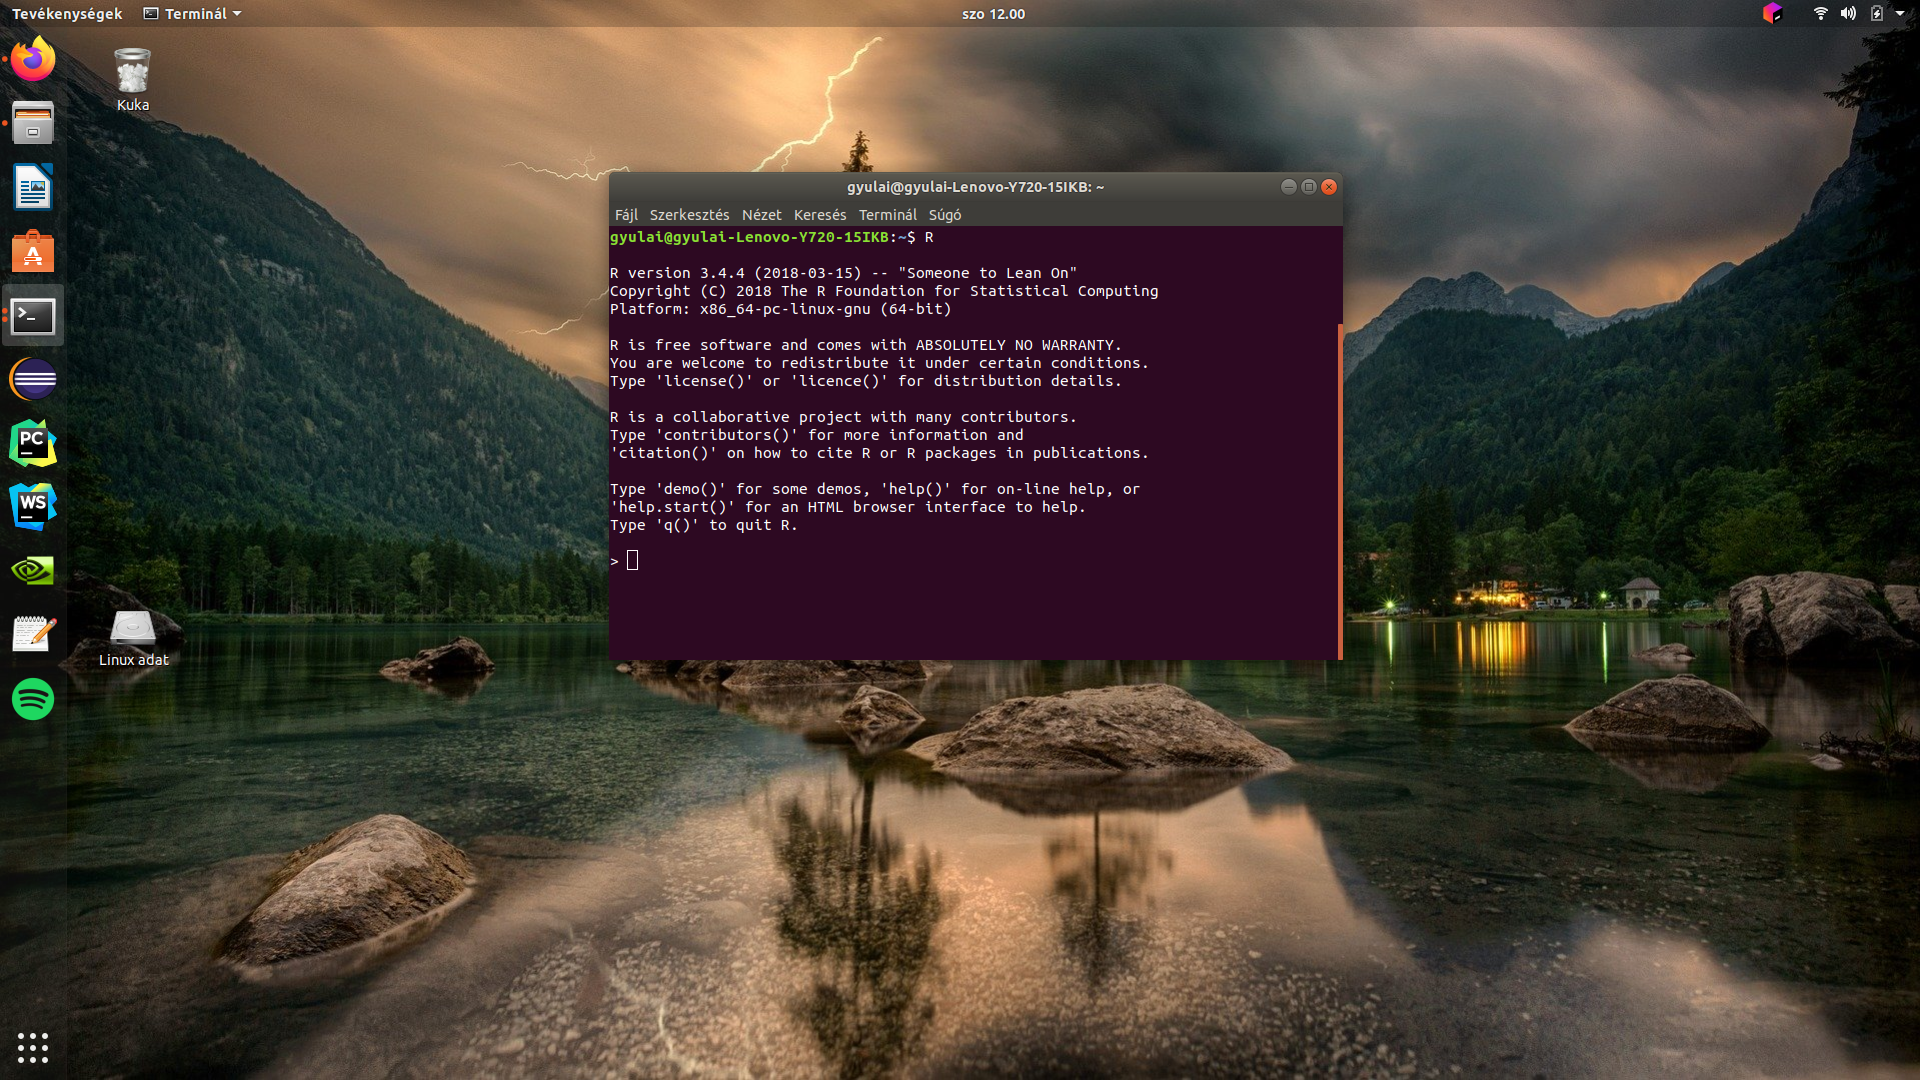
\includegraphics{img/R_screen.png}
\caption{alt text}
\end{figure}

A \textbf{GNU R} egy ingyenes szoftvercsomag, melyet elsődlegesen a
statisztikai számítások során alkalmaznak. Az \textbf{R} nem csak egy
programcsomag hanem egy programozási nyelv is egyben. Az R-t ahogy már
említettem statisztikai problémák megoldásánál érdemes használni, de a
nyelv egy nagy előnye, hogy nyílt forráskódú és ezáltal nagyon sok
csomag készült hozzá és ez kibővíti a képességeit több irányba is. Az R
elérhető Microsoft Windowsra, Linuxra, és Apple MacOS-re is. Az R is
képes importálni és exportálni az adatokat a leginkább használt
fájltípusokból, mint a CSV vagy XLS.

Weboldala: https://www.r-project.org/

    \subsubsection{Wolfram: Mathematica, Wolfram
Alpha}\label{wolfram-mathematica-wolfram-alpha}

    \paragraph{Wolfram Alpha}\label{wolfram-alpha}

\begin{figure}
\centering
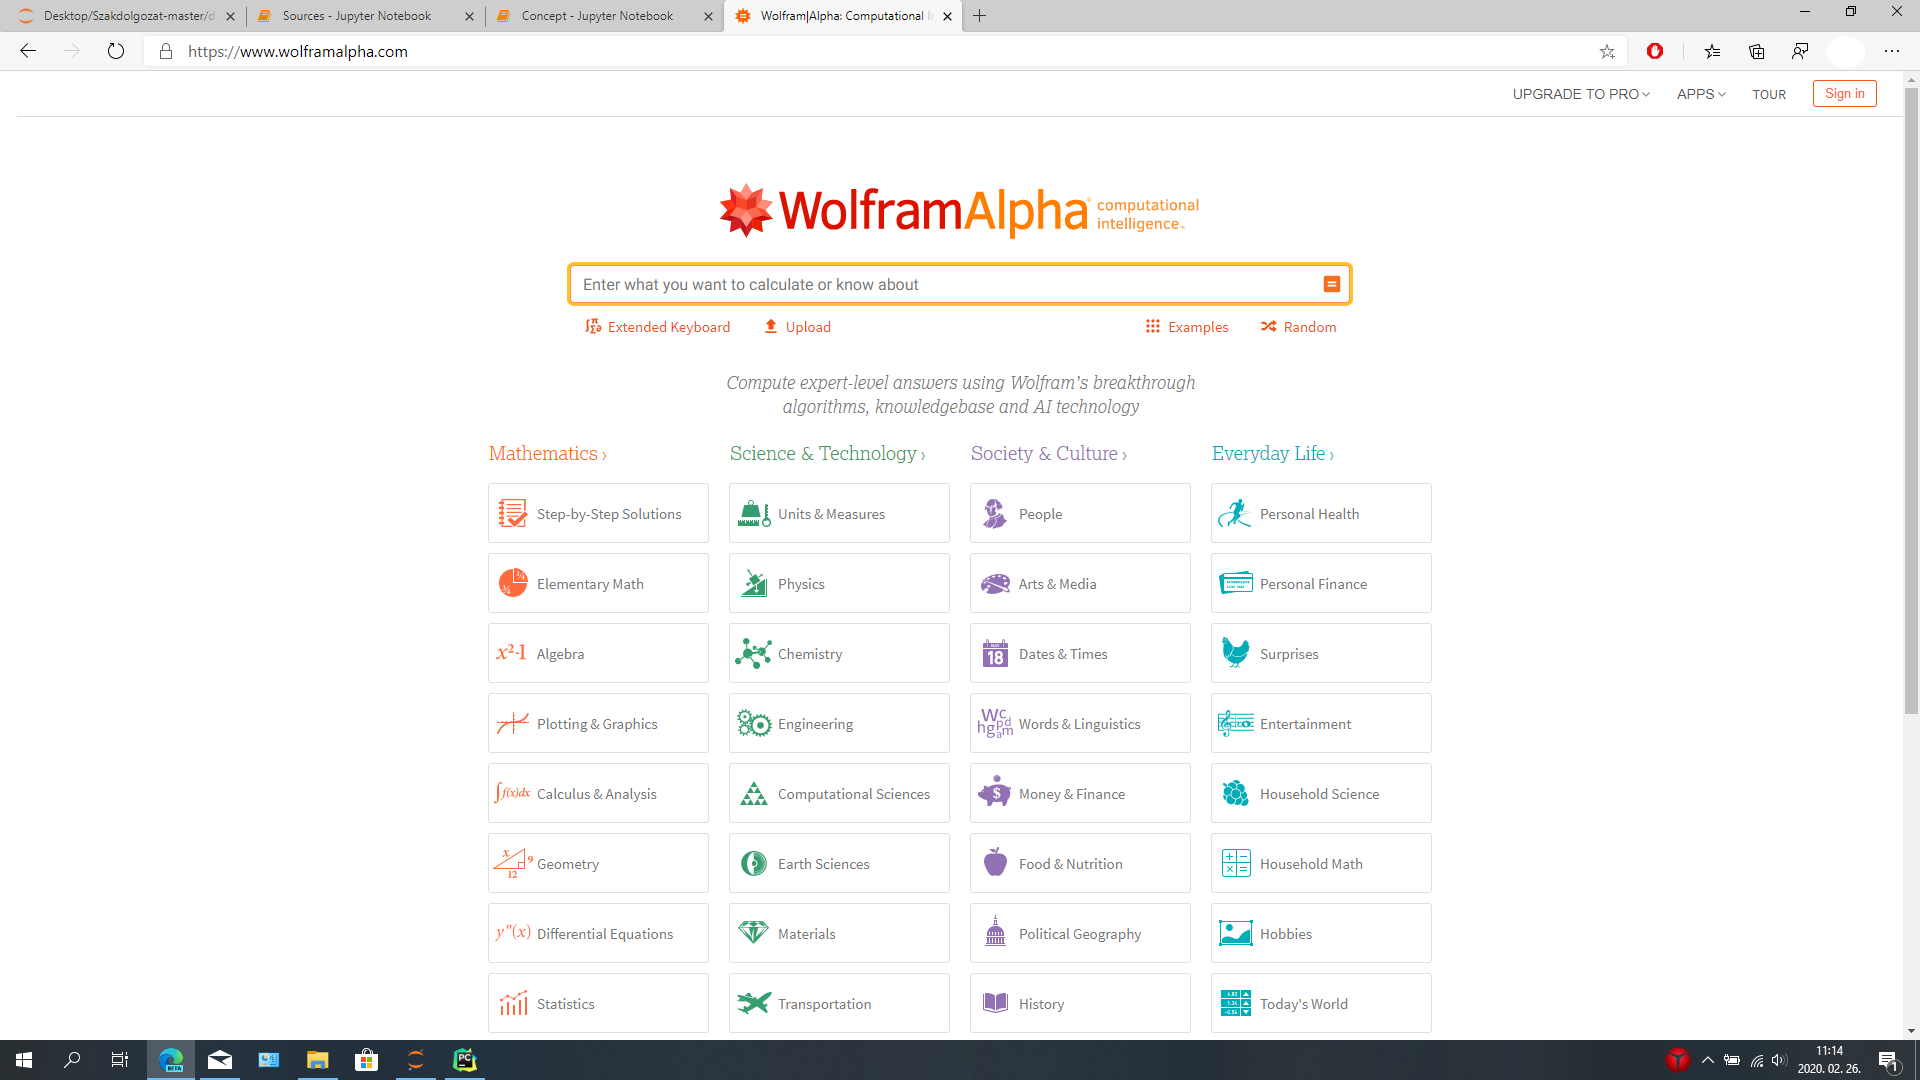
\includegraphics{img/alpha_screen.png}
\caption{alt text}
\end{figure}

A Wolfram Alpha nem is igazán egy szoftvercsomag inkább egy probléma
megoldó szoftver, melyet a Wolfram fejleszt és mely ötvözi a természetes
nyelv feldolgozást, az adatbányászatot és a dinamikus programozást,
ezáltal talál a megadott problémára megoldást. Az Alpha mögött óriási
adatbázis van. Létezik ingyenes megvalósítása mely elérhető a
weboldalán, illetve van egy Wolfram Alpha Pro elnevezésű változata is,
mely többet nyújt de fizetni kell érte. Az Alpha a fejlesztőknek
rengeteg API-t (\emph{Application programming Interface}, magyarul
alkalmazásprogramozási interfész) nyújt melynek egy része ingyenes, egy
részéért viszont szintén fizetni kell.

Weboldala: https://www.wolframalpha.com/

\paragraph{Wolfram Matematica}\label{wolfram-matematica}

A Matematica szintén a Wolfram által fejlesztett matematikai
programcsomag, a Matlab-hoz illetve a Maple-höz hasonlóan rengeteg
területet lefed. A Wolfram nevezetű szimbólikus programozási nyelvet
használja, mely az eddigiektől nagyon eltérő. A program csomag szintén
nem ingyenes. Elérhető Microsoft Windowsra, Linuxra, és Apple MacOS-re
és itt is találunk diák kedvezményt. Ha nem szeretnénk megvenni a teljes
csomagot, vagy nincs elég erős számítógépünk hozzá, akkor elérhető a
Matematica Cloud amire elő lehet fizetni egy évre, és csak egy böngésző
és internet kapcsolat szükséges hozzá. Az Alpha és a Matematica is
támogatja az adatok importálását és exportálását népszerű formátumú
fájlokba.

Weboldala: https://www.wolfram.com/mathematica/

    \subsection{Python eszközkészlet}\label{python-eszkuxf6zkuxe9szlet}

    A szakdolgozatban a Python nyelvet fogom használni és azon belül is
nagyrészben a Jupyter munkafüzetben dolgozom. Ahhoz, hogy pythonban
tudjunk dolgozni szükségünk van egy Python értelmezőre. Ez értelmezi a
kódot és hajtja azt végre. Több fajta Python interpreter létezik. A
legelterjedtebb a CPython mely C-ben és Python-ban íródott, ez a
referencia interpreter és ebből indul ki a többi interpreter is. Van
interpreter mely engedi hogy Java nyelvű kódot használjunk, és olyan is
mely a Python kódot lefordítja C vagy C++ nyelvű kóddá, vagy éppen olyan
is ami JavaScript-et vagy Java kódot varázsol a mi kis Python kódunkból.

Mivel Jupyter munkafüzetet használok, így használom az IPython nevezetű
shellt is. Mi is az az IPhyton? Az IPhyton, mint már említettem egy
shell ami tartalmazza a Jupyter kernelét és támogatja különböző
interpreterek használatát. Itt most a referencia CPython interpretert
használom majd. Ezen felül támogatja az IPhyton az interaktív adat
vizualizációt, interaktív elemek beépítését a munkafüzetbe, valamint a
párhuzamosítást is ha szükség lenne rá, illetve támogat különböző GUI
toolkiteket is. Az Adatok vizualizációjáért a fent már említett
Matplotlib csomag lesz felelős.

Ahhoz, hogy programozzunk valamilyen nyelven, kell valamilyen szöveg
szerkeztő vagy IDE és ez a Pythonnal sincs másképp. Pythonhoz elérhető
több nagytudású IDE is, mint a Spyder, Jupyter, Pycharm.

Kezdjük a Jupyterrel. Ez egy open-source web-alkalmazás mely olyan
dokumentumok létrehozását, szerkeztését, megosztását teszi lehetővé
melyben a programkódok lefuttathatóak, ezáltal olyan interaktív
dokumentumot készíthetünk melyben a programok bemutathatóak és a kapott
adatok könnyen vizualizálhatóak. A Jupyter több mint 40 programozási
nyelvet támogat.

Használhatjuk akár a Spyder-t is ami eg IDE kifejezetten Pythonhoz.
Főleg tudományos célú használatra készült és mint a Jupyter az IPythont
használja. mint minden IDE-t könnyű telepíteni és elkezdeni vele
dolgozni. Az Anaconda platformon belül ingyenesen érhető el.

Harmadik fejlesztő eszközünk a Pycharm, amit a JetBrains fejleszt.
Létezik egy ingyenes Community Edition és egy megvásárolható
Professional Edition. A Professional Edition sokkal több funkciót
támogat a Community Edition-el szemben, például a Jupyter notebookok
szerkeztését és megtekintését. A Pycharm azoknak kimondottan előnyös
akik használtak már valamilyen másik JetBrains által fejlesztett IDE-t,
hiszen a megszokott kezelő felülettel fognak találkozni.

\Chapter{Telepítés}

Ha szeretnénk Python-ban programozni ahoz szükségünk van egy
szövegszerkesztőre vagy integrált fejlesztő környezetre a Python
értelmezőn túl. A python értelmező ingyenesen elérhető a python
weboldaláról. A népszerűbb linux disztribúciók, mint az Ubuntu, Debian,
Linux Mint ...stb, már magába foglalja az értelmezőt ezért telepíteni
sem kell. A csomagok kezeléséhez szükségünk van a \texttt{pip} nevű
csomagkezelőre is. A \texttt{pip} segítségével tudjuk telepíten
lokálisan vagy globálisan a felhasználni kívánt csomagokat is melyek
előre megírt program könyvtárak tulajdonképpen, melyeket fel
használhatunk ahoz, hogy ne mindent nekünk kelljen implementálni. Ilyen
csomagok a Numpy, Matplotlib, Scipy, vagy a Jupyter notebook is melyeket
használok a későbbiekben.

    \subsection{Python telepítése}\label{python-telepuxedtuxe9se}

    Első lépésként le kell töltenünk a python értelmezőt a megfelelő
operációs rendszerünkre. Windows alatt a telpítőbe konfigurálhatjuk mit
telepítsünk, és azt is, hogy csak a saját felhasználónknak vagy pedig
mindenkinek szeretnénk telepíteni, útóbbihoz rendszergazdai jogosultság
szükséges.

Unix-szerű rendszereken sem sokkal nehezebb a dolgunk bár operációs
rendszerenként és disztribúciónként eltérések mutatkoznak.

A forráskódból való telepítéshez először is le kell tölteni a forrást,
szintén a python weboldaláról, majd kicsomagolni ezek után elnavigálunk
egy terminálban a mappába melybe kicsomagoltunk és futtatnunk kell a
configure nevezetű bash scriptet (\textbf{./configure} paranccsal tudjuk
megtenni). Miután végzett kiadjuk a \textbf{make} parancsot mellyel
elkezdődik a fordítási folyamat és felépül az alkalmazás esetünkben a
CPython értelmező. A következő lépés a \textbf{make test} mely
ellenőrzi, hogy minden rendben ment, majd jöhet a \textbf{sudo make
install} mellyel telepítjük az értelmezőt (make install előtt ott van a
sudo így láthatjuk hogy ehez szükségünk lesz root jogra (superuser)).

\emph{Megjegyzés:} - \emph{Itt ha a fordítás vagy a telepítés során
hibába ütközünk valószínüleg hiányzik valamilyen csomag a
számítógépünkről amit telepítenünk kell, ha ez megtörtént, újra le kell
futattni a parancsot amiben a hibát kaptuk és folytatódhat a folyamat
tovább.}

\begin{itemize}
\item
  \emph{Egyes linux disztribúciók rendelkeznek előre telepített
  értelmezővel, így felesleges telepíteni azt, ellenőrizzük le először,
  hogy telepítve van-e. Illetve némely linux disztribúció (főleg a
  debian alapúak mint, Debian, Ubuntu, Linux mint) különbséget tesz a
  python2 és python3 közözótt előbbit terminálból \textbf{python} míg
  utóbbit \textbf{python3} paranccsal érjük el és ez igaz a pip
  csomagkezelőre is, tehát, ha python3-al dolgozunk akkor a
  \textbf{pip3}-al tudunk hozzá csomagokat telepíteni.}
\end{itemize}

    A \texttt{pip} az új Python változatokban már a Python részeként
telepítésre kerül.

    \subsection{pip}\label{pip}

    A pipet egyszerűen lehet használni terminálban vagy windwos
parancssorban begépeljük hogy pip (vagy pip3) és megadjuk a csomag nevét
amit szeretnénk telepíteni: - \emph{pip somePackage} - \emph{python pip
-m somePackage}

Esetleg csinálhatunk olyat is, hogy összeírjuk a csomagokat egy
szövegfájlba (soronként egy csomagot) és telepítjük a - \emph{pip -r
csomagnevek.txt}

parancs segítségével.

pip weboldala: https://pip.pypa.io/en/stable/

    \subsection{Anaconda}\label{anaconda}

    A telepítés egy egyszerűsített változata, ha telepítjük az Anaconda
környezetet. Az Anaconda egy tudományos, gépi tanulásos platform,
melyben összegyűjtöttek több, mint 7500 python és R csomagot, melyeket
egyszerűen grafikus kezelő felület mellett telepíthetünk,ezen kívül
biztosít még IDE-ket (Spyder, Visual Studio Code) illetve a Jupyter
notebookot melyben ez a dolgozat is írodott. Az Anaconda telepítése
egyszerű. Felmegyünk a weboldalára, letöltjük és telepítjük Windows
alatt mind a 32 és 64 bites verzió támogatott míg Mac OS alatt
választhatunk grafikus vagy parancssoros telepítő között, Linux alatt
pedig támogatott az IBM Power 8 és 9 architektúrája is, az x86-64
mellett.

    \subsection{Jupyter munkafüzet}\label{jupyter-munkafuxfczet}

    A Jupyter notebookról még csak említés szintjén volt szó, most nézzünk
bele kicsit mélyebben mi is ez. A Jupyter notebook tulajdonképpen egy
nyílt forráskódú web alkalmazás mely lehetőséget nyújt arra, hogy olyan
interaktív dokumentumokat készítsünk és osszunk meg, melyek egyszerre
tartalmaznak futtatható kódokat és magyarázó szöveget, vizualizációkat.
A legelterjedtebben Python nyelvvel használják de támogat több, mint 40
programozási nyelvet köztük a C++, R, Ruby, julia és Calysto scheme
programozási nyelveket és a notebook ideális adat vizualizációra,
numerikus számításokhoz, gépi tanuláshoz és statisztikai modellekhez.

Maga a munkafüzet egy json szintaktikáju .ipynb kiterjesztésű fájl mely
úgynevezett cellákból áll. A celláknak vannak típusai: -
\textbf{markdown:} a markdown cellákban lehet a szöveget írni különböző
formázási lehetőségekkel. A markdown cellák támogatják a HTML elemeket
és a Latex matetmatikai módját, illetve más leíró nylevekből is vett át
egy két dolgot. - \textbf{code:} a code cellákban helyezhetjük el a
kódunkat melyet le szeretnénk futtatni - \textbf{heading:}
tulajdonképpen egy markdown cella csak rak a jupíter egy \#-ot az
elejére ami a legnagyobb headinget jelöli - \textbf{raw:} egy cella mely
nem kerül formázásra

A munkafüzet az IPython shellt használja, amely lehetővé teszi nekünk
ezt és az interaktív widget-ek használatát is a munkafüzetben, melynek a
segítségével így akár a kódunk paramétereit is megváltoztathatjuk.


\Chapter{NumPy hatékonyságának vizsgálata}

\section{Vektor és mátrix
műveletek}\label{vektor-uxe9s-muxe1trix-mux171veletek}

\subsection{Vektor műveletek:}\label{vektor-mux171veletek}

    Pythonban a \emph{NumPy} csomag használatával könnyedén definiálhatunk
vektorokat és mátrixokat. Ahhoz, hogy használhassuk előtte telepíteni
kell majd be kell a pip csomagkezelővel, majd az alábbi módon lehet
importálni:

\begin{python}
import numpy as np
\end{python}

    Ez a szintaktikája pythonban egy csomag inportálásának az \texttt{as}
operátor után aliast adhatunk a csomagnak, így megkönyítve a
használatát. Alias megadása nem kötelező.

    Ebben. esetben \texttt{np}-vel tudunk hivatkozni a \emph{NumPy}
csomagra. A csomagból az \texttt{array} metódus segítségével hozhatunk
létre vektorokat.

\begin{python}

\end{python}


    Üres vektort a következőképpen készíthetünk: az \texttt{empty}
metódusban meg kell adni szögletes zárójelek között egy dimenziót
(például: \texttt{{[}1,\ 3{]}} ez azt jelenti 1 sort és 3 oszlopot
szeretnénk), és esetlegesen megadhatunk neki egy adattípust, hogy milyen
adatokkal szeretnénk feltölteni.

    Itt főleg valmilyen numerikus adattípusra kell gondolni, hisz ezekkel
tudjuk elvégezni a vektor és mátrix műveleteket. Haszálhatjuk a python
beépített típusait mint az \texttt{int} vagy a \texttt{float}, de
használhatjuk a \emph{NumPy}-ban definiált kiegészített változatokat
amivel megadhatjuk azt például, hogy hány bájton tároljuk az adott
számot. Esetlegesen megadhatunk stringet és bool típust is ha szükség
van rá.

\begin{python}

\end{python}

\begin{python}

\end{python}

\begin{python}

\end{python}

\begin{python}

\end{python}

\begin{python}

\end{python}

\begin{python}

\end{python}

\begin{python}

\end{python}


    Ahogy láthatjuk, nem 0-ákkal tölti fel a vektort hanem valamilyen
memória szeméttel. Ennek az oka nagyon egyszerű: így gyorsabb, mint ha
nullázná az elemeket, de ha 0-ákkal szeretnénk feltölteni használhatjuk
a \texttt{zeros} metódust mely hasonló képpen működik mint az
\texttt{empty}:

\begin{python}

\end{python}

\begin{python}

\end{python}

    1-esekkel is feltölthetjük ehez a \texttt{ones}metódust használhatjuk:

\begin{python}

\end{python}

\begin{python}

\end{python}

    Létrehozhatunk egy bizonyos értékkel vagy pszeudóvéletlen (random)
számokkal feltöltött vektorokat is :

\begin{python}

\end{python}

\begin{verbatim}
[[0.22541693 0.47521003 0.90312494]]
[['aaa' 'aaa' 'aaa']]
\end{verbatim}

    A fent létrehozott \texttt{v1}, \texttt{v2}, \texttt{v3} vektorainkal
már egyszerűen elvégezhetőek a vektor műveletek, mint például az
összeadás:

\begin{python}

\end{python}

    vagy a kivonás:

\begin{python}

\end{python}

    vektoriális szorzás:

\begin{python}

\end{python}

    és a skaláris szorzás:

\begin{python}

\end{python}

    vagy számmal a való szorzás:

\begin{python}

\end{python}

    ha egyszerűen a összeszorozzuk a két vektort akkor a megfelelő hely lévő
tagokat szorozaz össze:

\begin{python}

\end{python}

    Transzponálhatjuk is a vektorainkat a \texttt{transpose} metódussal bár
vektorok esetén itt nem látványos:

\begin{python}

\end{python}

    Komolyabb műveletek mint a vektor normák kiszámítása is egyszerű. Vegyük
először az 1-es normát:

\begin{python}

\end{python}

    Itt használtuk a numpy \texttt{linalg} csomagját melyben előre
definiálva vannak a különbőző lineáris algebrához tartozó műveletek,
módszerek. Most nézzük a 2-es és a végtelen normát:

\begin{python}

\end{python}

    Mind itt a vektorműveleteknél és majd a mátrix műveleteknél sem árt
figyelni, hogy megfelelő dimenziójú vektorokat, mátrixokat adjunk meg a
műveletekhez, különben könnyen hibát vagy helytelen eredményt kaphatunk.

    \subsection{Mátrixok:}\label{muxe1trixok}

    A Mátrixok létrehozása is többféleképpen történhet hasonlóképpen mint a
vektoroknál. Legegyszerűbb módszer az ha megadjuk mi, hogy milyen
mátrixot szeretnénk vagy képezhetjük vektorokból is, estleg a fent
megismert \texttt{empty,\ zeros,\ ones,\ random.rand,\ full}
metódusoknak megadjuk a nekünk megfelelő dimenziókat.

   \begin{python}

\end{python}

\begin{verbatim}
m1
 [[1 2 4]
 [2 3 4]]
m2
 [[1 2 8]
 [2 3 9]]
m3
 [[1 2]
 [2 3]
 [4 5]]
m4
 [[1 2]
 [3 4]]
\end{verbatim}

\begin{python}

\end{python}

\begin{python}

\end{python}

    A \texttt{reshape}-nél vigyázni kell, hogy pontosan akkora elemszámú
mátrixot adjunk meg mint amekkora a mostani mátrixunké, különben hibát
kapunk.

\begin{python}

\end{python}

    Az \texttt{eye} metódu segítségével képezhetünk \(n*n\)-es
egységmátrixot, paraméterként a dimenziót kell megadnunk.

\begin{python}

\end{python}

\begin{verbatim}
[[1. 0. 0.]
 [0. 1. 0.]
 [0. 0. 1.]]
\end{verbatim}

    A vektorokhoz hasonlóan adhatjuk meg a mátrix műveleteket is, mint az
összeadást, kivonást, szorzást, normát:

\begin{python}

\end{python}

\begin{python}

\end{python}

\begin{python}

\end{python}

    Forbenius norma:

\begin{python}

\end{python}

    Végtelen norma:

\begin{python}

\end{python}

    1-es norma:

\begin{python}

\end{python}

    2-es norma

\begin{python}

\end{python}

    A transzponálás is hasonlóan működik:

\begin{python}

\end{python}

\begin{python}

\end{python}

    Egy négyzetes mátrix determinánsát is egyszerűen és gyorsan
kiszámíthatjuk a \texttt{linalg.det} metódussal:

\begin{python}

\end{python}

\begin{python}

\end{python}

\begin{python}

\end{python}

    Egy elemet az \texttt{item} metódussal tudunk kiválasztani, de figyelni
kell, mert az indexelés 0-tól kezdődik:

\begin{python}

\end{python}

    A mátrixokat feldarabolhatjuk a \texttt{hsplit} és \texttt{vsplit}
metúdusok segítségével. A \texttt{hsplit} oszlopok mentén, míg a
\texttt{vsplit} sorok mentén vágja el a megadott mátrixot.

\begin{python}

\end{python}

\begin{python}

\end{python}

\begin{python}

\end{python}

    Használhatjuk vágásra az \texttt{{[}{]}} operátorokat is, ha csak egy
paramétert adunk meg neki akkor az adott indexű sort kapjuk vissza, ha
használjuk a \texttt{:} operátort akkor megadhatunk neki intervallumot
is, hogy hanyadik sornál kezdje, megadhatunk neki lépésközt is illetve
részeket is kivághatunk egy adott mátrixból

\begin{python}

\end{python}

    Ha adunk meg neki lépésközt, akkor az az utolsó paraméter. Pl: az egész
mátrix minden párátlan számú sorának és oszlopának a közös elemei.

\begin{python}

\end{python}

    \subsection{Mátrix felbontások}\label{muxe1trix-felbontuxe1sok}

    \subsubsection{LU felbontás}\label{lu-felbontuxe1s}

    Mátrixok LU felbontásásval kinyerhetjük a felső- ,alsóháromszög
mátrixot. Pythonban erre használható a\texttt{Scipy.linalg.lu} metódus
ami a \texttt{SciPy} tudományos csomagban találhatunk meg ami egy
kiegészítése tulajdon képpen a \texttt{NumPy}-nak. Először telepíteni és
importálni kell ezt a csomagot és utána használatba lehet venni. Az
\texttt{lu} metódus végeredményként visszaadja az alsó-, felső-, és a
permutáció mátrixokat.

\begin{python}

\end{python}

    \begin{verbatim}
[[ 1.20000000e+01  1.30000000e+01  1.40000000e+01  1.50000000e+01]
 [ 0.00000000e+00  1.00000000e+00  2.00000000e+00  3.00000000e+00]
 [ 0.00000000e+00  0.00000000e+00 -4.44089210e-16 -9.99200722e-16]
 [ 0.00000000e+00  0.00000000e+00  0.00000000e+00  5.55111512e-16]]
    \end{verbatim}

    \subsubsection{Cholesky felbontás}\label{cholesky-felbontuxe1s}

    A Cholesky féle felbontásra is találunk beépített metódust a
\texttt{Numpy}-ban \texttt{cholesky} néven a \texttt{linalg} csomagban.
Cholesky felbontásnál vigyázni kell hogy a mátrixunk szimmetrikus legyen
és pozitív definit ellenben hibaüzenetet kapunk. Ugyan ez megtalálható a
\texttt{SciPy} csomagban is és a különbség az, hogy a \texttt{NumPy}-ban
lévő metódus az alsó-, addig a \texttt{SciPy}-ban lévő a felsőháromszög
mátrixot számolja.

\begin{python}

\end{python}

\begin{python}

\end{python}

    A fenti kód hibát eredményezett, mert a megadott mátrix nem volt pozitív
definit. A következő cellában már pozitív definit mátrixra van példa.

    \begin{python}

\end{python}

    De akár megírhatjuk a saját felbontó függvéníünket is:

   \begin{python}

\end{python}

    Mint ahogy láthajuk a metódus megadja egy közelítő megoldását a cholesky
felbontásnak.

\section{Lineáris
egyenletrendszerek}\label{lineuxe1ris-egyenletrendszerek}

    \subsection{Általánosan a lineáris
egyenletredszerekről}\label{uxe1ltaluxe1nosan-a-lineuxe1ris-egyenletredszerekrux151l}

    A lineáris egyenletrendszer egy többismeretlenes egyenletrendszer
melyben az ismeretlenek az első hatványon vannak.

    Egy \(n\) egyenlet és \(m\) változó esetén az egyenletrendszer általános
alakja a következő:

    \[
x_{1,1} + x_{1,2} + \dots + x_{1,m} = b_{1}\\
x_{2,1} + x_{2,2} + \dots + x_{2,m} = b_{2}\\
\vdots\\
x_{i,1} + x_{i,2} + \dots + x_{i,m} = b_{i}\\
\vdots\\
x_{n,1} + x_{n,2} + \dots + x_{n,m} = b_{n}\\
\]

    Aztmondjuk hogy az egyenlet rendszer alulhatárolt, hogyha \(n<m\) és
túlhatárolt, hogyha \(n>m\). Négyzetesnek nevezzük ha \(m=n\). Az
egyenletrendszer geometriai tartalmát az alábbi módon írhatjuk le:

    Az \(R^n\) euklideszi tér \(d\in R^n\) normálvektorú és \(x_0 \in R^n\)
ponton átmenő hipersíkját az

\[ (x - x_0)^Td=0\]

egyenletet kielégítő \(x \in R^n\) pontok határozzák meg.

    Az \(Ax=b\) egyenletrendszert felírhatjuk ilyen formában is:

    \[ 
a_{1}^Tx= b_1\\
a_{2}^Tx= b_2\\
\vdots\\
a_{n}^Tx= b_n\\
\]

    ahol \(a_{i}^T={a_{i1}, \dots a_{im}}\).

    Innen láthatjuk, hogy az egynletrendszer megoldása az \(m\) hipőersík
közös része, ennek megfelelően 3 megoldás lehetséges: 1. lehetőség:
nincs megolás 2. lehetőség: pontosan egy megoldása van 3. lehetőség:
végtelen sok megoldás van

    \paragraph{\texorpdfstring{\emph{Egynetrendszer
konzisztenciája:}}{Egynetrendszer konzisztenciája:}}\label{egynetrendszer-konzisztenciuxe1ja}

    \emph{Ha az \(Ax=b\) egyenletrendszernek legalább egy megoldása létezik
konzisztensnek nevezzük. Ha nem létezik egyetlen megoldása sem, akkor az
egyenletrendszer inkonzisztens.}

    \subsection{Lineáris egyenletrendszerek megoldása Pythonban, NumPy
csomag
segítségével}\label{lineuxe1ris-egyenletrendszerek-megolduxe1sa-pythonban-numpy-csomag-seguxedtsuxe9guxe9vel}

    Egy egyenletrendszert megoldani pythonban nem nehéz. A \texttt{NumPy}
tartalmazza a \texttt{solve} metódust mellyel könnyedén megoldható
egy-egy lineáris egyenletrendszer. A \texttt{solve} a \texttt{NumPy}
linalg csomagjában található, paramáterként várja az \(A\)
együtthatómátrixot és a \(b\) megoldásvektort. Nézzük is meg:

Vegyünk először egy egyszerű egyenletrendszert, mint ez: \[
    2x_1 + 9x_2 + 8x_3 + 7x_4= 7\\
    3x_1 - 2x_2 + 6x_3 + 4x_4= 4\\
    5x_1 + 8x_2 + 4x_3 + 7x_4= 2\\
    6x_1 + 9x_2 + 10x_3 + 2x_4= 6
\]

ezután importáljuk a numpy csomagot

\begin{python}

\end{python}

    Miután ezzel megvagyunk hozzuk létre az együttható métrixunkat és a
megoldás vektorunkat:

\begin{python}

\end{python}

    Majd használjuk a \texttt{solve} metódust

\begin{python}

\end{python}

\begin{python}

\end{python}

    A solve az Intel Math Kernel Library-ben megtalálható LAPACK gesv rutint
használja.

    A futás időt is kiírattam itt, hogy később össze lehessen vetni a
beépített és az általam implementált algoritmust. Az \texttt{allclose}
és\texttt{dot} metódusok segítségével pedig le is ellenőrízhetjük az
eredményt.

\begin{python}

\end{python}

\begin{python}

\end{python}
        
    Ilyen egyszerű az egész, de ha nem szeretnénk az előre megírt metódust
alkalmazni akkor definiálhatunk saját magunk is nekünk tetsző megoldó
metódust is. Például implementálhatjuk a Gauss módszert is. Ám mielőtt
ezt megnéznénk vessünk egy pillantást a ciklusokra pythonban csak, hogy
érthető legyen a kód.

    \paragraph{Rang}\label{rang}

    Egy lineáris egyenletrendszer csak akkor megoldható ha az A matrixunk
rangja megyegyezik a {[}A,b{]} mátrix rangjával ilyenkor az
egyenletrendszerünknek pontosan egy megoldása van. Ezt pythonban a
következő képpen tudjuk ellenőrizni:

\begin{python}

\end{python}

   \begin{python}

\end{python}

    Amint látjuk a két rang megegyezik ezáltal megoldható az itt látható
egyenlet rendszer.

    \paragraph{Ciklusok pythonban:}\label{ciklusok-pythonban}

    Pythonban is megtalálható a \texttt{for} és a \texttt{while} ciklus. A
\texttt{for} végig iterál egy iterálható objektumon ami pythonban lehet
egy tömb, string vagy az általunk kreált iterálható struktúra.

\begin{python}

\end{python}

    Ha klasszikus értelemben szeretnénk használni (tehát egy ciklus változót
léptetni egy kezdő értéktől egy végértékig) használnunk kell a
\texttt{range} metódust mely generál egy tömböt a megadott paraméterek
alapján. Három paramétere van, az első a kezdő érték, a második a
végérték és a harmadik a lépésköz. A \texttt{range} esetében figyelni
kell, mert a végéertékig generálja a számokat ezért a végérték nem
szerepel az általa vissza adott tömbben.

   \begin{python}

\end{python}

    A \texttt{while} működése nem tér el a többi általános célú programozási
nyelvben megszokottól. Amíg a megadott feltételünk igaz addig maradunk a
ciklusban.

\begin{python}

\end{python}

\begin{python}

\end{python}

    Nézzük még meg az \texttt{if} elágazást is mely megvizsgál egy logikai
kifejezést és annak értéke szerint ágaztatja el a programot.

  \begin{python}

\end{python}

    És akkor lássuk a Gauss módszer implementációját:

    \paragraph{Gauss módszer pythonban:}\label{gauss-muxf3dszer-pythonban}

   \begin{python}

\end{python}

    Láthatjuk futás időben elég közel van a numpyban lévő megoldáshoz. De
nem kapunk olyan pontos eredményt.

    Tegyünk most kis kitérőt a számítási munkára ezt valahogyan mérni kell,
hogy megtudjuk adni egyes algoritmusoknak a műveletigényét és ennek a
mértékegysége a flop. Egy régi flop az a számítási munk ami az
\(s=s+x*y\) művelet (egy összeadés és egy szorzás) elvégzéséhez kell, 1
új flopp pedig az a számítási munka mely egyetlen művelet (mindegy az
hogy additív vagy multiplikatív) elvégzéséhez szükséges. Az új flop
bevezetését az indokolta, hogy a mai számítógépeken a multiplikatív és
az additív műveletek elvégzéséhez szükséges idő azonosnak tekinthető.

    A gauss módszer $\dfrac{n^3}{3} + O(n^2)$ addítív és ugyanennyi
multiplikatív műveletet igényel, így a művelet igénye:\(\dfrac {n^3}{3}+
O(n^2) \) régi flop és \(\dfrac {2n^3}{3}+ O(n^2) \) új flop.

    \paragraph{Főelem kiválasztás}\label{fux151elem-kivuxe1lasztuxe1s}

    A fenti algoritmus csak olyan mátrixokat képes megoldani amikben egyik
együttható sem nulla. Hogy képes legyen rá ki kell egészíteni főelem
kiválasztással. A főelem kiválasztás azt jelenti, hogy a sorokat úgy
cseréljük fel, hogy az aktuális pivot elemünk ne legyen nulla. A
főelemkiválasztás lehet részleges vagy teljes. Részleges főelem
kiválasztásnál a \(k\)-adik lépésben megkeressük a \(k\)-adik oszlop
elemei közül a maximális abszolút értékű \(a_{ik}\) együtthatót és ez az
\(j\)-edik sorban van akkor megcseréljük a \(j\)-edik és a \(k\)-adik
sort. Ezzel fogunk majd találkozni a gauss-Jordan módszer
implementációjánál. A teljes főelem kiválasztás során pedig a \(k\)-adik
lépésben megkeressük a mátrixban szereplő értékek közül a maximális
abszolút értékűt és ha ez a \(a_{ij}\) akkor a \(k\)-adik sort
felcseréljük az \(i\)-edikkel és a \(k\)-adik oszlopot is felcseréljük a
\(j\)-edikkel.

    \paragraph{Gauss-Jordan módszer
pythonban}\label{gauss-jordan-muxf3dszer-pythonban}

    Egy másik lehetséges módszer az egyenletrendszerek megoldására a
Gauss-Jordan módszerezt leimplementálhatjuk mi magunk is, de én most egy
másik csomagot a SymPy-t fogom segítségül hívni. Első lépésnek vegyük az
\(A\) mátrixunkat és a \(b\) vektorunkat, majd használjuk az A mátrixra
definiált \texttt{gauss\_jordan\_solve} mmetódust melynek paraméterként
a \(b\) vektort adjuk meg. A metódus két visszatérési értéke a megoldás
és a mátrix.

\begin{python}

\end{python}

    Fontos, hogy a Matrixot nem kompatibilis az np.arrayel, így az értékeket
nekünk kell áthelyezni.

    Van egy 4. módszer is a lineáris egyenlet rendszer megoldására a
\texttt{scipy} csomagban, ami az lu faktorizáción alapul. A metódus neve
pedig \texttt{lu\_solve} és az alábbi módon lehet használni:

\begin{python}

\end{python}

    Most lássunk egy összesítő táblázatot a 3 módszerről:

\begin{python}

\end{python}


 \section{Interpolációk}\label{interpoluxe1ciuxf3k}

    \subsection{Általánosan az
interpolációkról}\label{uxe1ltaluxe1nosan-az-interpoluxe1ciuxf3kruxf3l}

    Az interpolációk alapfeladata az, hogy egy \(f(x)\) függvény felvett
értékeit különböző \(x_1, x_2 x_3 \dots x_n\) pontokban ismerjük az
\([a,b](a=x_1, b=x_n)\) intervallumban és magát az \(f\) függvényt
szeretnénk közelíteni egy könnyen számolható \(h(x)\) függvénnyel,
amelyre fenáll, hogy \(f(x_i)=h(x_i)\). Az \({x_i}_{i=1}^n\) pontokat
interpolációs alappontoknak, a feltételt interpolációs feltételnek
nevezzük. Az interpolációs feltétel teljesülése esetén azt reméljük,
hogy az interpoláló \(h(x)\) függvény jól közelíti az \(f(x)\) függvényt
az \([x_i,x_i+1]\) intervallumokban. Itt a Lagrange, Hermit és Spline
interpolációkról fogok elsősorban írni.

    Legegyszerűbben interpolációt ai \texttt{interp1d} metódussal tudunk
végre hajtani. ez a metódus nem kér csak \(x,y\) értékeket és a
interpoláció módját. A metódus a scipy.interpolate csomagban található
meg.

\begin{python}

\end{python}

    \begin{center}
%    \adjustimage{max size={0.9\linewidth}{0.9\paperheight}}{output_4_0.png}
    \end{center}
    { \hspace*{\fill} \\}
    
    Látható az \texttt{interp1d} egy függvénnyel tér vissza aminek csak meg
kell adnunk az \(x\) értékeinket és vissza adja az eredményt. Ezek
használhatóak a legkönnyebben pythonban. fontos, hogy miután elvégeztük
az interpolációt adott pontokra a függvénynek azonos intervallumon de
több alpontot tartalmazó tömböt adjunk át kirajzolásnál, hogy szépen és
pontosan rajzolja ki a közelítő függvénytés.

    Míg az \texttt{interp1d} \(y=f(x)\) típusú függvényeket interpolál addig
ennek a metódusnak a párja az \texttt{interp2d} már az \(z=f(x, y)\)
tipusú egyenleteket tudja közelíteni. használata az
\texttt{interp1d}-hez hasonló.

\begin{python}

\end{python}

    \begin{center}
%    \adjustimage{max size={0.9\linewidth}{0.9\paperheight}}{output_7_0.png}
    \end{center}
    { \hspace*{\fill} \\}
    
    Másik egyszerűen használható metódus a numpy csomagban található
\texttt{interp1d}. Az \texttt{interp1d} esetében meg kell adni az \(x\)
és \(y\) értékeinket illetve egy olyan intervallumot az \([a,b]\)
intervallumon ami több alpontot tartalmaz. A megadott alpontok számától
függ a pontosság tehát lehetőleg elég sokat adjunk meg. Az
\texttt{interp1d} szakaszokra ad meg lineáris interpolácót.

\begin{python}

\end{python}

    \begin{center}
    %\adjustimage{max size={0.9\linewidth}{0.9\paperheight}}{output_9_0.png}
    \end{center}
    { \hspace*{\fill} \\}
    
    \subsection{Lagrange interpoláció}\label{lagrange-interpoluxe1ciuxf3}

    Legyenek a \(\phi_i\) bázisfüggvények a következők
\(\phi_1=1, \phi_2=x, \dots , \phi_n=x^{n-1}\) és legyenek
\(x_1, x_2,\dots, x_n\) alpontjaink és \(y_i=f(x_i)\) az alpontokhoz
tartozó függvény értékek. Ekkor a feladatunk az, hogy határozzuk meg a
legfeljebb n-1-ed fokú \(p\) polinomot amelyre igaz, hogy
\(p(x_i)=y_i\). Ez tulajdonképpen az alapfeladat a lényegi rész az, hogy
ezt a \(p\) polinomot hogyan állítjuk elő. A Lagrange féle előállítás a
következőképpen néz ki:

    \[
l_i(x)=\prod_{k=1, k\neq i}^n\frac{x-x_k}{x_i-x_k}
\] Majd ezekhez az \(l_i\) értékeket megszorozzuk a \(y_i\) értékeket és
megkapjuk a \(p\) polinomot. \[
p(x)=\sum_{i=1}^n y_il_i(x)
\]

    Ezáltal meg kapjuk az \(f(x)\) függvényünk közelítését a \(p(x)\)
polinom által. (\(f(x) \approx p(x)\))

    Pythonban a scipy.interpolate csomag \texttt{lagrange} függvényével
tudunk a lagrange interpolációt számolni. Figyelni kall hogy egy poly
nevű változóba tér vissza.

\begin{python}

\end{python}

    \begin{center}
    %\adjustimage{max size={0.9\linewidth}{0.9\paperheight}}{output_15_0.png}
    \end{center}
    { \hspace*{\fill} \\}
    
    Látszik a pontosság itt is fögg a megadott alpontok számától. Bár a
lagrange interpolációnak létezik pythonos implementációja numerikusan
unstabil ezért ha mindenféleképpen ezt szeretnénk használni érdemesebb a
saját implementációnkat elkészíteni.

    \subsection{Spline interpoláció}\label{spline-interpoluxe1ciuxf3}

    Spline interpoláció esetén is megvannak az \(x_i\) pontjaink és \(y_i\)
függvényértékeink és ezek mellett keressük azt az \(S(x)\) függvényt
mely teljesíti az alábbi feltételeket: \[
S(x)= S_i(x)\quad x\in[x_i, x_{i+1}]\\
S(x_i)= y_i\quad (i=1, \dots, n)\\
S_i(x_{i+1})= S_{i+1}(x_{i+1})\quad (i=1, \dots, n-2)\\
\]

    Az első feltétel megfogalmazza,hogy szakaszokból áll a függvényünk, a
második megmondja, hogy valóban interpoláló függvény az \(S(x)\)
függvényünk és a harmadikkal a folytonosság van definiálva az \([a,b]\)
intervallumon.

    A spline meghatározásánál felírunk \(n\) darab \(k\)-ad fokú polinomot
ebből látszik, hogy az ismeretlenek száma \(n(k+1)\). Az első és a
harmadik feltételből következik az, hogy a feltételek száma
\((k+1)n-(k-1)\), ugyanis \(k-1\) db simasági feltétel a \(n-1\) belső
pontban ebből jön az, hogy \((n-1)(k-1)\) és \(2n\) interpolációs
feltétel. Összesen \((n-1)(k-1)+2n=(k+1)n-(k-1)\) és ebből látszik, hogy
hiányzik a spline egyértelműségéhez még \(k-1\) darab feltétel. Ezeket a
végpontokra szokták megadni.

    Vegyük először a lineáris spline interpolációt ebben az esetben a
\(k=1\) és a három feltétel egyértelműen meghatározza. Minden
\([x_k, x_{k+1}]\) intervallumon: \[
S_k(x_k)=a_kx_k+b_k=y_k \\
S_k(x_{k+1})=a_kx_{k+1}+b_k=y_{k+1}\\
\] Ebből a kétismeretlenes egyenletrendszerből meghtározható \(a_k\) és
\(b_k\).

    Beszélhetünk még kvadratikus splineokról is ebben az esetben \(k=2\) és
\(k-1 = 1\) feltétel hiányzik a spline egyértelmű felírásához. Ezt a
feltételt általában az intervallum elején vagy végén a derivált
megadásával szokás teljesíteni. Az így felvázolt esetben az egymás
melletti intervallumokra Hermite interpolációt alkalmazva meghatározható
a spline.

    Gyakorlatban azonban a harmadfokú spline interpolációt használjuk
túlnmyómó részt és csak harmadfokú splineról beszélünk, viszont ezek
további feltételek felírását követelik meg: \[
S_i'(x_{i+1})= S_{i+1}'(x_{i+1})\quad (i=1, \dots, n-2)\\
S_i''(x_{i+1})= S_{i+1}''(x_{i+1})\quad (i=1, \dots, n-2)\\
S''(x_{1})= A_n \quad \textrm{és} \quad S''(x_{n})=B_n
\]

    Pythonban használhatjuk a harmadfokú splinet is ehez elő kell készíteni
a scipy.interpolate csomagban megtalálható \texttt{splprep} metódussal
majd utána tudjuk használni a \texttt{splev} metódust ami a harmadfokó
splinet adja vissza.

    Először vegyünk egy függvényt és pár alpontot legyen most ez a sinus
függvény és próbáljuk ezt közelíteni spline-al.

\begin{python}

\end{python}

    \begin{center}
    %\adjustimage{max size={0.9\linewidth}{0.9\paperheight}}{output_26_0.png}
    \end{center}
    { \hspace*{\fill} \\}
    
    Látható hogy a harmadfokó spline jól közelíti a függvényünket hiszen
nagyjából lefedi és a megadott pontokban felveszi az értéket a megadott
értékeket.

    \subsection{Hermite interpoláció}\label{hermite-interpoluxe1ciuxf3}

    A harmadik interpoláció amit csak megemlítek az a Hermite interpoláció.
Hermite interpoláció esetén ugyan úgy megvannak az
\(x_0, x_1, \dots, x_n \in [a,b])\) pontjaink, mint eddig és vannak
mellé $m\_0, m\_1, \dots, m\_k \quad (k\leq n)$ multiplicitások is,
úgyhogy $\sum_{i=0}^k m_i=n+1$, továbbá adottak az
\(f^{(j)}(xi)=y_{ij}, \quad (i=0,\dots,k \quad\textrm{és}\quad j=0,\dots,m-1)\)
értékek is. Feladatunk az, hogy megkeressünk egy n-ed fokú P polinomot
melyre igaz hogy,: \[
P^{(j)}(xi)=y_{ij}, \quad (i=0,\dots,k \quad\textrm{és}\quad j=0,\dots,m-1)
\]

\subsection{Sajátérték,
Sajátvektor}\label{sajuxe1tuxe9rtuxe9k-sajuxe1tvektor}

    A mátrixok sajátértékéhez és sajátvektorához szükségünk lehet a komplex
számok halmazára is. Egy ilyen komplex számokból álló mátrixot a valős
számokból állóhoz hasonlóan \(\mathbb{C}^{mxn}\)- el jelöljük
\((\mathbb{R}^{mxn} \subset \mathbb{C}^{mxn})\). nézzük először a
sajátvektor és a sajátérték definícióját:

Legyen \(A \in \mathbb{C}^{nxn}\) tetszőleges mátrix. A
\(\lambda \in \mathbb{C}\) számot az \(A\) mátrix sajátértékének és az
\(x \in \mathbb{C}^n \quad (x\neq0)\) vektort pedig \(\lambda\)
sajátértékhez tartozó sajátvektornak nevezzük, ha

\[
Ax=\lambda x.
\]

    Fontos, hogy egy mátrix sajátértékeinek összeségét a mátrix spektrumának
nevezzük és a spektrumból a mátrix fontos tulajdonságait lehet kiolvasni
például: - Egy négyzetes mátrix akkor és csak akkor nemszinguláris ha
egyik sajátértéke sem nulla. - Egy mátrix akkor és csak akkor pozitív
definit, ha minden sajátértéke pozitív.

    A sajátértékeket úgy kaphatjuk meg ha megoldjuk a karakterisztikus
egyenletet ami a következő: \[
\phi(\lambda)=det(A-\lambda i)=0
\]

ezt kifejtve megkapjuk a \(\lambda\) változó \(n\)-ed fokú polinomját
azaz a:

\[
\phi(\lambda)=(-1)^n\lambda^n+p_{n-1}\lambda^{n-1}+\dots+p_1\lambda+p_0
\]

karakterisztikus polinomot. komplex számok körében ennek a polinomnak
pontosan \(n\) db zérushelye van tehát egy \(A\in \mathbb{C}^{nxn}\)
mátrixnak pontosan \(n\) darab sajátértéke van, ha figyelembe vesszük a
multiplicitásokat.

    És most térjünk rá a Pythonban való megvalósítására. A sajátértékeket és
vektorokat a numpy.linag csomagban található \texttt{eig} metódussal
tudjuk kiszámolni az alábbi módon.

\begin{python}

\end{python}

    Az \texttt{eig} egy \(nxn\)-es mátrixot vár és két vektorral tér vissza
az első (w) tartalmazza a sajátértékeket, a második (v) pedig a saját
vektorokat normalizát alakban. Az i-edik (w{[}i{]}) sajátértékhez az
i-edik (v{[}:i{]}) a oszlop tartalmazza a sajátvektort.

    A numpy.linag csomagban találunk még egy \texttt{eigvals} mely csak a
sajátértékeket számolja ki és ugyanúgy egy \(nxn\)-es mátrixot vár
paraméterként.

\begin{python}

\end{python}

    Ezek a metódusok a \_geev LAPACK rutint használják.


\section{Matplotlib és a Legkissebb négyzetek
módszere}\label{matplotlib-uxe9s-a-legkissebb-nuxe9gyzetek-muxf3dszere}

    

    Ahogy a szoftvereszközök bemutatásánál már volt róla szó, az adatok
vizualizálása nagyon fontos, hisz egy-egy ábráról könyebb adatokat
leolvasni, mint nagy táblázatokból vagy egyéb adastruktúrákból.
Pythonban a \texttt{matplotlib} felel ezeknek az ábráknak a
létrehozásához. Nézzük is meg hogyan is kell.

    Először vegyünk egy egyszerű példát például bizonyos \(x\) értékekhez
rendeljünk hozzá \(f(x)=y\) értékeket.

\begin{python}

\end{python}

    Látható, tehát a matplotlib plot hívásásval tudjuk kirajzopltatni az
ábráinkat, melynek az első paramátere a értelmezési tartomány, a második
az értékkészlet, és további paramáterként meglehet neki adni a jelölés
formáját illetve feliratokat a label paraméter segítségével. Az
értékeket megadhatjuk függvény segítségével is :

\begin{python}

\end{python}

    \begin{center}
    %\adjustimage{max size={0.9\linewidth}{0.9\paperheight}}{output_6_0.png}
    \end{center}
    { \hspace*{\fill} \\}
    
    Megváltoztathatjuk a színét is az adott ábránknak illete több függvényt
is ábrázolhatunk egyszerre.

\begin{python}

\end{python}

    
    \begin{verbatim}
<Figure size 2775x1575 with 1 Axes>
    \end{verbatim}

    
    Az előző kódrészben importáltam a \texttt{figure}- t a matplotlib
csomagból. Ennek segítségével képesek vagyunk mbeállítani az ábra
alapvető beállításait, mint itt a méretet, de beállíthatjuk a háttér és
szélek színeit vagy a felbontást (dpi).\\
A tengelyeket is elnevezhetjük könnyedén a matplotlib \texttt{ylabel} és
\texttt{xlabel} metódusaival és adhatunk címet is az ábránknak a
\texttt{title} metódussal:

\begin{python}

\end{python}

    \begin{center}
    %\adjustimage{max size={0.9\linewidth}{0.9\paperheight}}{output_10_0.png}
    \end{center}
    { \hspace*{\fill} \\}
    
    Az előző példában használtam a \texttt{**} operátort ami egy egyszerű
módja hogy valamit valamelyik hatványra emeljünk.

    A matlotlib segítségével létrehozhatunk hisztogrammokat is

\begin{python}

\end{python}
        
    \begin{center}
    %\adjustimage{max size={0.9\linewidth}{0.9\paperheight}}{output_13_1.png}
    \end{center}
    { \hspace*{\fill} \\}
    
    Adatainkat egy ploton belül töbféleképpen is megjeleníthetjük

\begin{python}

\end{python}

    \begin{center}
    %\adjustimage{max size={0.9\linewidth}{0.9\paperheight}}{output_15_0.png}
    \end{center}
    { \hspace*{\fill} \\}
    
    Ilyen esetben a a jelőlő pontokat a marker, míg a színt a color
paraméterrel tudjuk megváltoztatni

    \subsection{Legkissebb négyzetek
módszere}\label{legkissebb-nuxe9gyzetek-muxf3dszere}

    És most, nézzünk meg egy példát a legkissebb négyzetek módszerén, hogy
való használatban is lássuk a matplotlib előnyét.

    Feladatunk az, hogy kapott mérési eredményekre ráillesszünk egy
egyenest. Adottak az értékek ez egy \(y \in R^n\) és a hozzájuk tartozó
helyek $x\in R^n$, és ezek alapján keressük a \(y= a_0+a_1x\)
egyenest melyre a
$\sum_{i=0}^{N[y_i-(a_0+a_1 x_i)]}2$
minimális. Szerencsénkre erre is tartalmaz beépített metódust a
\texttt{NumPy}. A \texttt{linalg} csomagban található \texttt{lstsq}
metódus megadja az egyenest amire szükségünk van.

\begin{python}

\end{python}

    \begin{center}
    %adjustimage{max size={0.9\linewidth}{0.9\paperheight}}{output_20_0.png}
    \end{center}
    { \hspace*{\fill} \\}
    
    \subsection{3D plotting}\label{d-plotting}

    A Matplotlib megengedi számunkra az is, hogy 3 dimenziós ábrákat
készítsünk el. Ezek lehetnek felületek 3D-s térben elszórt pontok
esetleg függvények is. Ehhez szügségünk van a \textbf{mplot3d} csomagra
ami az \textbf{mpl\_toolkits} része.

    elsőnek nézzünk meg egy 3 dimensziós ívet:

\begin{python}

\end{python}

    \begin{center}
    %\adjustimage{max size={0.9\linewidth}{0.9\paperheight}}{output_24_0.png}
    \end{center}
    { \hspace*{\fill} \\}
    
    Az ábbrán látható hogy a pontok által leírt ívet jeleníti meg egyetlen
vonalként a matplotlib de akár elhelyezhetjük rá az adott diszkrét
pontokat is.

\begin{python}

\end{python}

    \begin{center}
    %\adjustimage{max size={0.9\linewidth}{0.9\paperheight}}{output_26_0.png}
    \end{center}
    { \hspace*{\fill} \\}
    
    Megtehetjük azt is hogy cak a pontokat helyezzük el a 3D-s térben.

\begin{python}

\end{python}

    \begin{center}
    %\adjustimage{max size={0.9\linewidth}{0.9\paperheight}}{output_28_0.png}
    \end{center}
    { \hspace*{\fill} \\}
    
    Egy felületet megjeleníthetünk többféleképpen is a \textbf{wireframe}
segítségével egy háló szerűen, míg a \textbf{surface} használatával
egybefüggő felületként. Figyelni kell míg az előzőekben a

\begin{python}

\end{python}

    \begin{center}
    %\adjustimage{max size={0.9\linewidth}{0.9\paperheight}}{output_30_0.png}
    \end{center}
    { \hspace*{\fill} \\}
    
\begin{python}

\end{python}

    \begin{center}
    %\adjustimage{max size={0.9\linewidth}{0.9\paperheight}}{output_31_0.png}
    \end{center}
    { \hspace*{\fill} \\}
    
    És akkor nézzük a surface-t

\begin{python}

\end{python}

    \begin{center}
    %\adjustimage{max size={0.9\linewidth}{0.9\paperheight}}{output_33_0.png}
    \end{center}
    { \hspace*{\fill} \\}
    
    3D plottingnál csak kirajzolja a matplotliba az ábrákat nem interaktív,
nem tudjuk forgatni, de beállíthatjuk a szöget amelyből nézni szeretnénk
az ábrát.

\begin{python}

\end{python}

    \begin{center}
    %\adjustimage{max size={0.9\linewidth}{0.9\paperheight}}{output_35_0.png}
    \end{center}
    { \hspace*{\fill} \\}
    
    Sok más lehetőséget is kínál a matplotlib példáúl megjeleníthetünk
3d-ben 2-ds adatokat vagy csinálhatunk 3d-s hisztogrammot több adattal,
de a fent említettek talán a legfontosabbak és legtöbbet használtak.

    \subsection{Interaktív widgetek
jupiterben}\label{interaktuxedv-widgetek-jupiterben}

    Az interaktív plotokról nem szeretnék sokat beszélni hiszen ezek
készítését nem a Python, hanem a Jupyter notebook és a IPython kernel
teszi lehetővé. Ha mégis ezeket használnánk akkor az
\texttt{interact}segítségével tudunk interaktív dolgokat csinálni
számoltatni mondjuk több adatra megnézni egy egy függvény képét. itt a
példában különböző hatvány függvényeket lehet megnézni és a csúszka
segítségével lehet beállítani a hatvány kitevőt.

\begin{python}

\end{python}

    
    \begin{verbatim}
interactive(children=(IntSlider(value=1, description='y', max=30, min=1), Output()), _dom_classes=('widget-int…
    \end{verbatim}

    
    Vagy akár a minta számot is beállíthatjuk egy ilyen csúszkával és ezzel
a pontosságot tudjuk szabályozni.

\begin{python}

\end{python}

    
    \begin{verbatim}
interactive(children=(IntSlider(value=1, description='y', max=200, min=1), Output()), _dom_classes=('widget-in…
    \end{verbatim}

    
    Saját tapasztalatom az hogy minden értékre kirajzolja az ábrát
interaktív dolgok esetén ezért nagy megadott értékre eljutni eltelhet
egy kis időbe

    Az interaktivitásnak sok formája van használhatunk ilyen csúszkákat, de
vannak még igaz, hamis értékekre \texttt{Checkbox}-ok, szöveges
bevitelre alkalmas mező(\texttt{Text}), lenyíló
lista(\texttt{Dropdown}), illetve eddig nem volt külön kiemelve a
csúszkának két fajtája van az egészekre használható \texttt{IntSlider},
illetve a lebegő pontos számokkal dolgozó \texttt{FloatSlider}. Egy
interact híváshoz használhatunk akár több paramétert is. Itt egy kis
példa példáúl egy text mezőre mely összead két számot.

\begin{python}

\end{python}

    
    \begin{verbatim}
interactive(children=(Text(value='', description='a'), Text(value='', description='b'), Output()), _dom_classe…
    \end{verbatim}

    
    Fontos megjegyezni, hogy a beírt dolgok szövegként kerülnek átadásra,
úgyhogy szükség lehet kasztolásra számok esetén.

\begin{python}

\end{python}

    
    \begin{verbatim}
interactive(children=(IntSlider(value=1, description='hatvanykitevo', max=20, min=1), IntSlider(value=2, descr…
    \end{verbatim}

    
    Megvalósításából fakadóan ezek az interaktív eszközök használhatóak 3D
plotoknál illetve más helyeken is.

    Például 3D-s esetben megvalósítható velük a plot forgatása is.

\begin{python}

\end{python}

    
    \begin{verbatim}
interactive(children=(IntSlider(value=0, description='angle1', layout=Layout(width='600px'), max=360), IntSlid…
    \end{verbatim}

    
    Mint látható a layout tulajdonsággal meg lehet változtatni az egyes
widgetek megjelenését. A tulajdonságokat CSS szerűen adhatjuk meg.
Fontos hogy a \texttt{Layout}-ot is importálni kell használat előtt.


    % Add a bibliography block to the postdoc
    
    \section{Numerikus deriválás és Numerikus
integrálás}\label{numerikus-derivuxe1luxe1s-uxe9s-numerikus-integruxe1luxe1s}

    \subsection{Numerikus deriválás}\label{numerikus-derivuxe1luxe1s}

    A numerikus deriválás alapfeladata az, hogy az analitikusan ismeretlen
vagy nehezen számolható, esetleg csak diszkrét pontokban ismert
\(f:D(\subseteq \mathbb{R})\rightarrow \mathbb{R}\) függvény
deriváltjának kiszámítás egy vagy több pontban.

Többféleképpen indulhatunk neki csinálhatunk egy interpolációt mely
közelít az \(f\) függvényünkhöz és akkor az interpolációnk \(k\)-adik
deriváltja fog közelíteni az \(f\) függvényünkhöz \(k\)-adik
deriváltjához.

Ha \(f \in C^2[a,b]\) akkor felírhatjuk rá a másodfokú Taylor polinomot
amiből kifejezhetjük az alábbi összefüggést:

\[
f'(x)\approx \frac{f(x+h)-f(x)}{h}
\]

Melynek hibája \(O(h)\). A harmadfokú taylor polinommal még pontosabb
közelítést kaphatunk:

\[
f'(x)\approx \frac{f(x+h)-f(x-h)}{2h}
\]

Másodfokú deriváltra alkalmazott összefüggések:

\[
f''(x)\approx \frac{f(x)-2f(x+h)+f(x+2h)}{h^2}
\]

\[
f''(x)\approx \frac{f(x+h)-2f(x)+f(x-h)}{h^2}
\]

A második képlet a centrális differencia formula. Mind a két képlet
hibája \(O(h^2)\)

ezeknek az implementációja:

\begin{python}

\end{python}

    \begin{center}
    %\adjustimage{max size={0.9\linewidth}{0.9\paperheight}}{output_3_0.png}
    \end{center}
    { \hspace*{\fill} \\}
    
    Interpolációkkal való közelítéshez használható a Newton, Lagrange és a
Spline interpoláció is.

    \subsection{Numerikus integrálás}\label{numerikus-integruxe1luxe1s}

    Numerikus integrálásnál a Newton-Leibnitz formulából indulunk ki. Ha
vagy egy \(f\) függvény és az Riemann integrálható \([a,b]\)-n és itt
létezik primitív függvénye, akkor

\[
I=\int^b_a f(x)dx=F(b)-F(a)
\]

Ezt a képletet viszont csak akkor tudjuk alkalmazni ha létezik \(f\)-nek
primitív függvénye egyébként numerikus integrálást kell alkalmaznunk.
Numerikus integrálást úgy tudunk alkalmazni, ha az \(f\) függvényünket
közelítjük egy \(p\) interpolációs polinommal és ezáltal a határozott
integrál értékét általános formában közelítjük:

\[
I=\int^b_a f(x)w(x)dx \approx \int^b_a p(x)w(x)dx,\quad \textrm{ ahol a $w(x)\geq0$ egy tetszőleges súlyfüggvény}
\]

    Integráláshoz találunk előre megírt függvényeket a scipy.integrate
csomagban amik a \texttt{quad}, \texttt{dblquad}, \texttt{tplquad}. A
sima \texttt{quad} egy általános esetekben használható függvény a
\texttt{dblquad} a \texttt{quad}-hoz hasonló de kétszeres integrálást
végez, míg a \texttt{tplquad} pedig háromszorosan integrál.

\begin{python}

\end{python}

    Vannak persze egyébb algoritmusok is melyeket lehet használni, ilyen a
Lagrange formula vagy a zárt vagy nyitott Newton-Cotes formulák is, ezek
mellett ott vannak még a Téglalap és Trapéz formulák is. A Newton-Cotes
formulákra visszavezethető a Simpson és az érintő formula is.

    Nézzük meg ezek közül először a két legegyszerűbbet a Téglalap
formulákat és a Trapéz módszert. Kezdjük a Téglalap formulákkal. Az
\(f\) függvény integrálját szeretnénk az \([a,b]\) intervallumon, legyen
\(h=(b-a)/n\) a lépésköz ekkor az első téglalap formula a következő:

\[
I^{(1)}= h  \sum^{n-1}_{j=0}y_j
\]

a második pedig:

\[
I^{(2)}= h  \sum^{n}_{j=1}y_j
\]

és van egy harmadik is:

\[
I^{(3)}= h  \sum^{n}_{j=1}y_{j-1/2}
\]

Látszik hogy a formulák a téglalapokat illesztenek a függvényre és ezek
területének az összege adja meg az integrál értékét.

\begin{python}

\end{python}

    
    \begin{verbatim}
interactive(children=(Text(value='', description='numOfPoints'), Output()), _dom_classes=('widget-interact',))
    \end{verbatim}

    
    Látható hogy nem ugyan azt az eredményt adják, de elég sok alpont esetén
az egzakt megoldáshoz tartanak. A téglalap formula hibája az alpontok
számától függ lineárisan azaz \(O(h)\).

    Most nézzük a Trapéz módzser. A trapéz módzsernek van egy egyszerű és
egy összetett változata is. Először vegyük az egyszerűt. Ebben az
esetben 1 alpontunk van tehát \(h=1\). Legyen \(a=x_0\) és \(b=x_1\)
ekkor: \[
\int^b_a f(x)dx \approx \frac{y_0+y_1}{2}h
\]

\begin{python}

\end{python}


    \begin{center}
    %\adjustimage{max size={0.9\linewidth}{0.9\paperheight}}{output_14_1.png}
    \end{center}
    { \hspace*{\fill} \\}
    
    Látható nem ad pontos eredményt. most nézzük meg az összetett trapéz
módszert. Az Összetett trapéz módszer esetén már több alpontuk van tehát
\(h\geq 1\) és az alábbi képletet alkalmazzuk:

\[
\int^b_a f(x)dx \approx \sum^{n-1}_{j=0}\frac{x_{i+1}-x_i}{2}(y_i+y_{i+1})
\]

   \begin{python}

\end{python}

    Látható ez már sokkal pontosabb eredményt ad, mint az egyszerű trapéz
módszer.

    Folytassuk az érintő formulával. Az érintő formula egy nyílt
Newton-Cotes formula melyre:

\[
\int^b_a f(x)dx \approx (b-a)f( \frac{a+b}{2})
\]

Ez a formula úgy is értelmezhtő, hogy az \(f\) függvényünket a
középpontjához húzott egyenessel közelítjük az \([a,b]\) intervallumon,
és az egyenes alatti területet vesszük. ebből következik, hogy maximum
első fokú polinomig pontos. Gyakorlatban nem ezt a képletet szokták
alkalmazni, hanem az intervallumot felosztják n egyenlő részre és ezt a
képletet alkalmazzák:

\[
\int^b_a f(x)dx \approx \frac{(b-a)}{n}\sum^{n}_{i=1}f( a-\frac{h}{2}+ih)
\]

Nézzük meg ezek implementációját:

\begin{python}

\end{python}

    Az egyszerű érintő formula hiba becslése:

\[
\big| \int^a_b f(x)dx-(b-a) f \big( \frac{a+b}{2} \big)\big| \leq \frac {(b-a)^3M_2}{24}.
\]

    Végül jöjjön a Simpson formula mely egy zárt Newton-Coats formula melyre
\(n=2\). ennek is van egyszerő és összetett alakja. Az egyszerű alakhoz
3 alpontra van szükségünk \(x_1=a, x_1=\frac {a+b}{2}, x_2=b\) és
alakalmazzuk a három pontra támaszkodó Lagrange-féle interpolációs
polinomot:

\[
\int^b_a f(x)dx \approx \frac{b-a}{6} [f(a)+4f(\frac{a+b}{2})+f(b)]
\]

Az összetett Simpson formula esetén is az intervallumot felosztjuk \(n\)
egyenlő részre és akkor ilyen módon változik meg a képletünk:

\[
\int^b_a f(x)dx \approx \sum^{n-1}_{i=0}\frac{x_{i+1}-x_i}{6} [ f(x_i) + 4f( \frac{x_i+x_{i+1}}{2})+ f({x_{i+1}} ) ]
\]

És most nézzük meg az implementációt:

\begin{python}

\end{python}


    A Simpson formula hibája:

\[
\big|\int^a_b f(x)dx- S_n(f)\big| \leq \frac {M_4(b-a)}{32 \cdot 90}h^4 = \frac {M_4(b-a)^5}{2880n^4}
\]

\section{Hibák}\label{hibuxe1k}

    Mikor hibáról beszélünk akkor sok mindenre gondolhatunk, például egy
program írása közben kaphatunk futásidejű vagy fordításiidejű hibákat,
nincs ez másképp a való életben is lehet hiba ha megteszünk valamit vagy
ha éppen nem. Ez nincs másképp egy matematikai feladatnál sem. Ebben az
esetben az alábbi hiba típusokról beszélhetünk:

\begin{itemize}
\item
  Modellhiba: amikor a valóságnak csak egy közelítését használjuk egy
  feladat matematikat alakjának a felírásához.
\item
  Mérési vagy öröklött hiba: amikor a modell adatai a valós pontos
  értékeknek csak valamilyen közelítő értékei, ezek általában amérés
  pontosságától függnek
\item
  Műveleti és input hiba: ezek a hibák a számítógépen tárolt adatok
  számítógépen való ábrázolásánból adódó hibák. Ezek a számábrázolási
  hibák azért léphetnek fel, mivel a számítógépen a racionális számoknak
  is csak egy részhalmaza ábrázolható lebegő pontos aritmetikában. A
  műveletek elvégzésénél fel léphet kerekítés, túl- illetve
  alulcsordulás.
\item
  Képlethiba: amikor a végtelen eljárást véges számú lépés után
  leállítunk, közelítő eljárásokat alkalmazunk.
\end{itemize}

    \subsection{Számábrázolás}\label{szuxe1muxe1bruxe1zoluxe1s}

    \subsubsection{Egész számok:}\label{eguxe9sz-szuxe1mok}

Számítógenp az egész számokat előjeles vagy előjel nélküli bináris
számként lehet elképzelni, ezáltal jellemzhetőek a számjegyek számával.
Az egész számokat általában 2 vagy 4 byteon tároljuk el 2-es, 10-es vagy
16-os számrendszerben, ez az adott programozási nyelvtől függ. Az
egészekkel végzett aritmetikai műveletek gyorsabbak a lebegő pontos
számokkal végrehajtott aritmetikai műveleteknél és ezáltal egy
algortimus lefutását fel tudja gyorsítani a használatuk és emellett
hibamentesnek tekinthetőek ezek a műveletek. Használatuknál viszont
vigyázni kell és alaposan át kell gondolni mikor hasznájuk, mert
tulajdonképpen maradékosztályokban dolgozunk.

\subsubsection{Lebegőpontos számok:}\label{lebegux151pontos-szuxe1mok}

\begin{figure}
\centering
%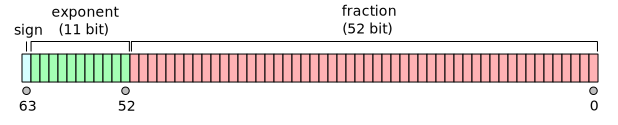
\includegraphics{img/IEEE_754.svg}
\caption{alt text}
\end{figure}

Lebegő pontos számok esetében a számítógépek egy véges számhalmazt
ábrázolnak és a számításokat is ezekkel a számokkal végzik el.
Álatalában a lebegőpontos aritmetikát használják. Ennek nézzük meg a
modelljét:

\paragraph{Definíció:}\label{definuxedciuxf3}

A nem nulla lebegőpontos számok általános alakja:

\[
\pm a^k(\frac{m_1}{a}+\frac{m_2}{a^2}+\dots+\frac{m_t}{a^t}),
\]

ahol \(a>1\) a számábrázolás alapja, \(\pm\) az előjel, \(t>1\) a
számjegyek száma és \(k\in \mathbb{Z}\) a kitevő.

Az \(m_1\) számjegy normalizált, \((1\leq m_1 \leq a-1)\) ez garantálja
a az ábrázolás egyértelműségét. A többi
számjegy:\(1\leq m_i \leq a-1 \quad (i=2,3,\dots,t)\). A nulla az nem
normalizált tehát \(k=0, m_1=m_2=\dots=m_t=0\) és az előjele általában
\(+\). A számábrázolás alpaja itt is lehet 2, 10, 16 vagy akár más is,
átalában a programozási nyelven múlik melyiket használja. Pontosság
szempontjából: - \(t=8\) egyszeres pontosság - \(t=16\) dubla pontosság

A géptől és pontosságtól függően \(m\) tárolására \(32,64\) vagy \(128\)
bit áll rendelkezésünkre (ez rendre \(4,8,16\) byte). Ezzel párhuzamosan
nő a \(k\) értékkészlete, és adott pontosság mellett:

\[
 L \leq k \leq U.
\]

A legnagyobb ábrázolható szám:

\[
M^\infty=a^U(1-a^-t)
\]

A legkissebb pedig:

\[
-M^\infty
\]

A lebegőpontos számok a \([-M^\infty,M^\infty]\)-beli számok diszkrét
(racionális) részhalmazát alkotják és ez a részhalmaz a nullára nézve
szimmetrikus. A nullához legközelebb eső lebegő pontos szám:
\(\varepsilon_0=a^{L-1}\) és az \(\varepsilon_0\)-hoz legközelebb eső
szám pedig: \(\varepsilon_0(1+a^{1-t})\).

A gép relatív pontossága vagy másképpen a gépi epszilon a
\(\varepsilon_1=a^{1-t}.\)

    \subsection{Klasszikus hiba analízis}\label{klasszikus-hiba-analuxedzis}

\paragraph{Definíció:}\label{definuxedciuxf3}

Legyen \(A\) egy pontos értékt és legyen \(a\) ennek valamilyen
közelítése. A \(\Delta a=A-a\) mennyiséget a közelítés hibájának
nevezzük és a \(|\Delta a|=|A-a|\) pedig az abszolút hibájának. Azt a
\(\delta a\) értéket pedig abszolút hibakorlátnak nevezzük amelyre
fenáll, hogy \(|A-a|=|\Delta a| \leq \delta a\).

Az \(A\) szam valamilyen közelítő értékének a relatív hibája pedig a
\(\frac {\delta a} {A}\) mennyiség

Az additív műveletek abszolút hibákorlátja pedig a következőek:

\[
\delta(a+b)\leq \delta a+ \delta b \\
\delta(a-b)\leq \delta a+ \delta b
\]

Az multiplikatív műveletek abszolút hibákorlátjai:

\[
\delta(ab) \approx |a|\delta b +|b| \delta a \\
\delta(a/b) \approx  \frac {|a|\delta b +|b| \delta a}{|b|^2}
\]

Az aritmetikai műveletek relatív hibakorlátjai a következőek, feltéve
hogy a nevező sehol sem nulla és az additív műveleteknél az operandusok
megegyező előjelűek:

\[
\frac{\delta(a+b)} {|a+b|} =  max( \frac{\delta a}{|a|}, \frac{\delta b}{|b|} ) \\
\frac{\delta(a-b)} {|a-b|} = \frac{\delta a + \delta b} {|a-b|} \\
\frac{\delta(ab)} {|ab|} \approx \frac{\delta a}{|a|} + \frac{\delta b}{|b|} \\
\frac{\delta(\frac {a}{b})} {|\frac {a}{b}|} \approx \frac{\delta a}{|a|} + \frac{\delta b}{|b|}
\]

\Chapter{Megjelenítési módok}

Az eredmények megjelenítésére már a korábbiakban is sor került. Ez a fejezet külön egységként vizsgálja, hogy a Python, főként a \texttt{matplotlib} segítségével milyen segítséget ad az adatok vizualizálásához.

\Section{Egyszerű grafikonok rajzolása}
    
Ahogy a szoftvereszközök bemutatásánál már volt róla szó, az adatok
vizualizálása nagyon fontos, hisz egy-egy ábráról gyakran könnyebb adatokat
leolvasni, mint nagy táblázatokból vagy egyéb adastruktúrákból.
Python-ban a \texttt{matplotlib} függvénykönyvtárt használhatjuk ezeknek az ábráknak a
létrehozásához.

    Először vegyünk egy egyszerű példát, amelyben bizonyos \(x\) értékekhez
rendeljünk hozzá \(f(x) = y\) értékeket.
\begin{python}
import matplotlib.pyplot as plt
import numpy as np

x = np.zeros(20)
y = np.zeros(20)

for i in range(-9, 10):
    x[i] = i
    y[i] = pow(x[i], 2)
    
plot = plt.plot(x, y, "o")
\end{python}
    A \texttt{matplotlib} \texttt{plot} hívásával tudjuk kirajzoltatni az
ábráinkat, melynek az első paramátere a értelmezési tartomány, a második
az értékkészlet, és további paramáterként meg lehet neki adni a jelölés
formáját, illetve feliratokat a label paraméter segítségével.

Az értékeket megadhatjuk függvény segítségével is, például
\begin{python}
import matplotlib.pyplot as plt
import numpy as np

x = np.zeros(20)
y = np.zeros(20)

for i in range(-9, 10):
    x[i] = i
    
plot=plt.plot(x ,abs(x),"-", label='x abszolut erteke', markersize=10)
plot = plt.legend()

plt.show(plot)
\end{python}
Ennek az eredménye \aref{fig:abs-plot}. ábrán látható.

\begin{figure}[h!]
\centering
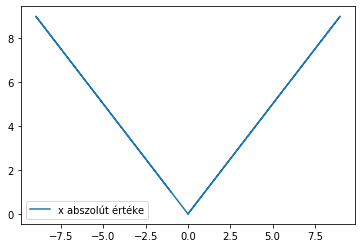
\includegraphics[scale=1.0]{img/abs-plot.png}
\caption{Függvény kirajzolása a \texttt{matplotlib} segítségével.}
\label{fig:abs-plot}
\end{figure}

    Megváltoztathatjuk a színét is az adott ábránknak, illete több függvényt
is ábrázolhatunk egyszerre, például
\begin{python}
import matplotlib.pyplot as plt
import numpy as np
from matplotlib.pyplot import figure

x = np.zeros(100)
d = -4
i = 0
while i < 100:
    x[i] = d;
    d = d + 0.1
    i = i + 1
    
plt.figure(figsize=(18.5, 10.5), dpi=150)
plot = plt.plot(x,np.cos(x), "-r", label='cos x')
plot = plt.plot(x,np.sin(x), "-g", label='sin x')
plot = plt.legend()
plt.show(plot)
\end{python}
Az eredmény \aref{fig:sin-plot}. ábrán szerepel.

\begin{figure}[h!]
\centering
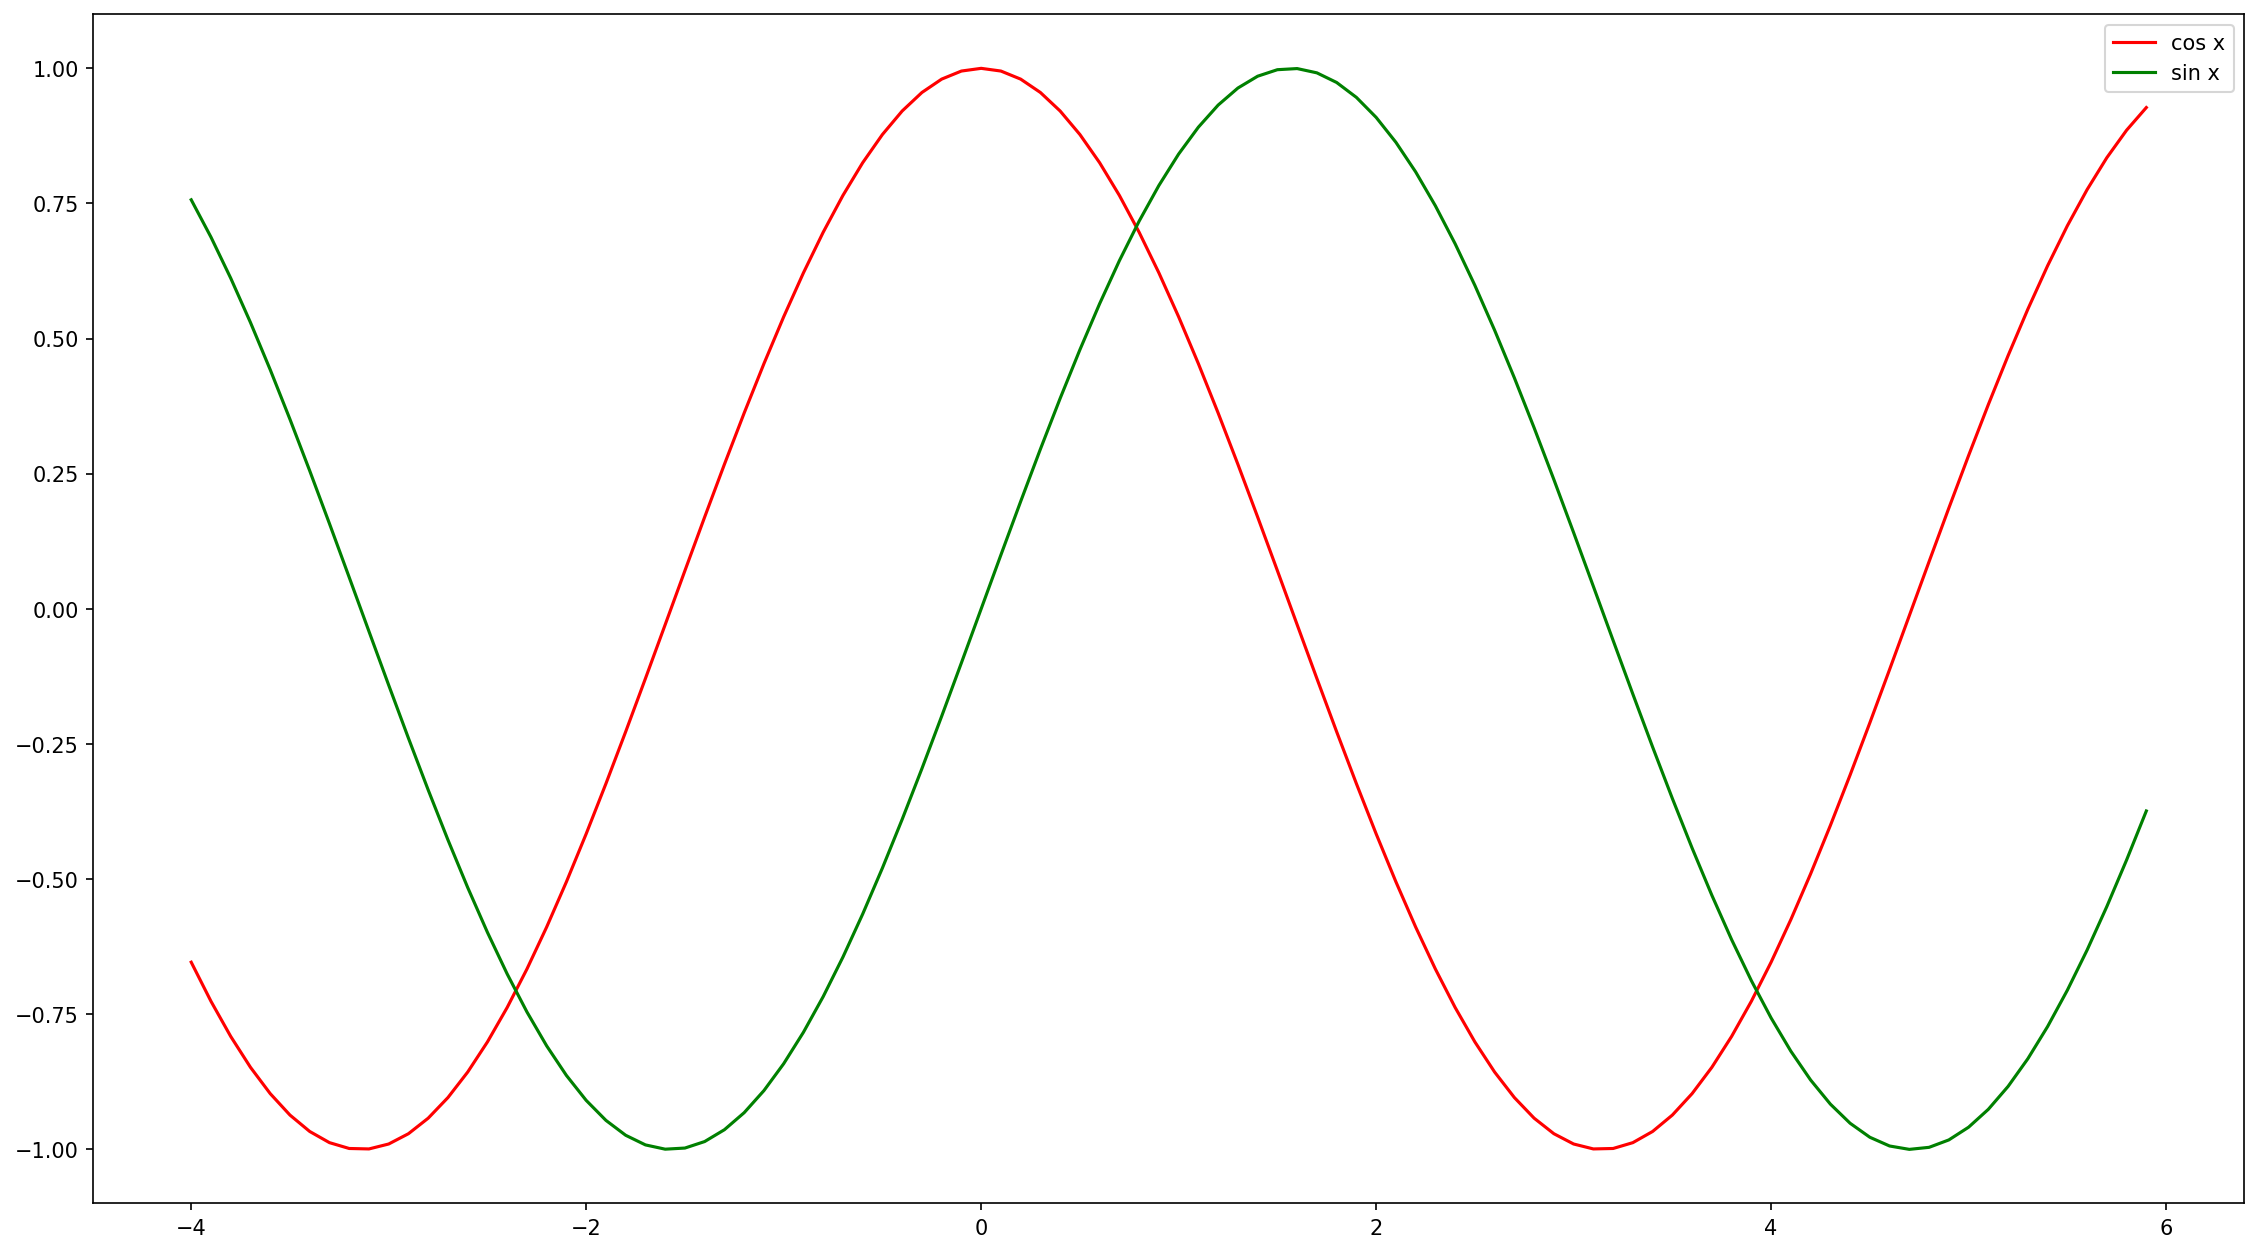
\includegraphics[width=\textwidth]{img/sin-plot.png}
\caption{Több függvény egyidejű kirajzolása.}
\label{fig:sin-plot}
\end{figure}

    Az előző kódrészben importáltam a \texttt{figure}-t a \texttt{matplotlib}
csomagból. Ennek segítségével képesek vagyunk beállítani az ábra
alapvető tulajdonságait, úgy mint például a méretet, de beállíthatjuk a háttér és
szélek színeit vagy a felbontást.

A tengelyeket is elnevezhetjük könnyedén a matplotlib \texttt{ylabel} és
\texttt{xlabel} metódusaival és adhatunk címet is az ábránknak a
\texttt{title} metódussal.

Létrehozhatunk hisztogrammokat is, továbbá adatainkat egy ploton belül töbféleképpen is megjeleníthetjük:
\begin{python}
test = ['1', '2', '3', '4', '5', '6']
points = [68, 70, 75, 76, 80, 78]

plt.figure(figsize=(18.5, 10.5), dpi=150)

plt.subplot(131)
plt.bar(test, points, color='b')
plt.subplot(132)
plt.scatter(test, points, marker='*', color='r')
plt.subplot(133)
plt.plot(test, points, color='black')

plt.show()
\end{python}
Az eredménye \aref{fig:multi-plot}. ábrán látható.

\begin{figure}[h!]
\centering
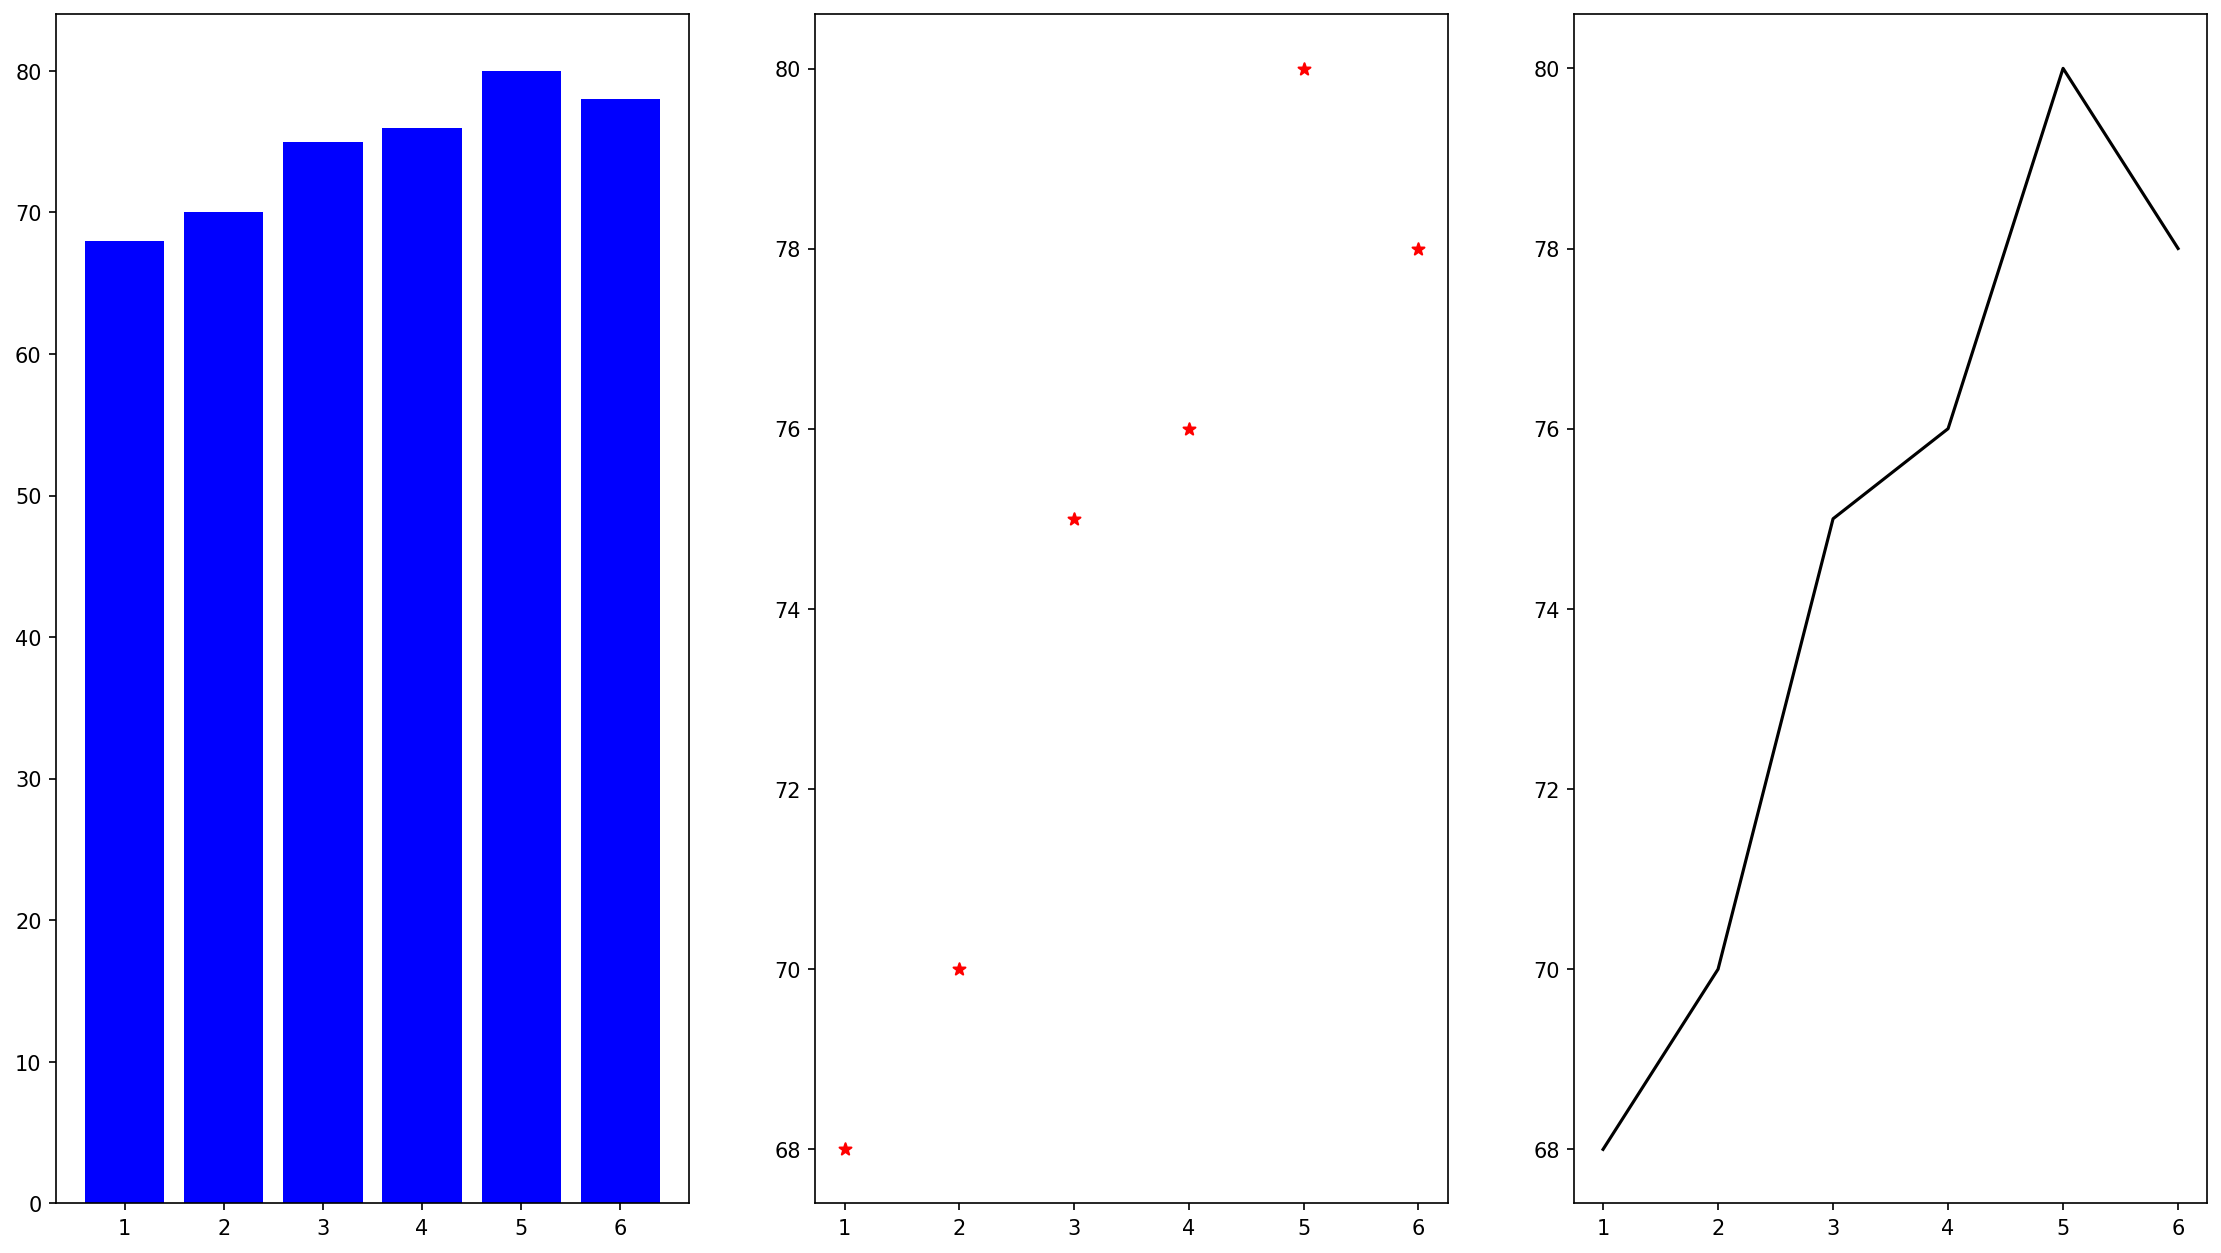
\includegraphics[width=\textwidth]{img/multi-plot.png}
\caption{Több grafikon megjelenítése egymás mellett.}
\label{fig:multi-plot}
\end{figure}
    
    Ilyen esetben a a jelőlő pontokat a \texttt{marker}, míg a színt a \texttt{color} paraméterrel tudjuk megváltoztatni.
    
\Section{Térbeli pontok szemléltetése}

    A Matplotlib megengedi számunkra az is, hogy térbeli pontokat képezzünk le ábráinkon. Ezek lehetnek felületek  térben elszórt pontjai vagy egyéb függvények is. Ehhez szügségünk van a \textbf{mplot3d} csomagra
ami az \textbf{mpl\_toolkits} része.
Először nézzünk meg egy térbeli ívet!
\begin{python}
import matplotlib.pyplot as plt
from mpl_toolkits.mplot3d import axes3d

fig = plt.figure(figsize=(18.5, 10.5), dpi=150)
ax = fig.add_subplot(111, projection='3d')

theta = np.linspace(-4 * np.pi, 4 * np.pi, 100)
z = np.linspace(-2, 2, 100)
r = z**3 + 1
x = r * np.sin(theta)
y = r * np.cos(theta)
ax.plot(x, y, z)
plt.show()
\end{python}
A kirajzolás eredménye \aref{fig:curve-1}. ábrán látható.

\begin{figure}[h!]
\centering
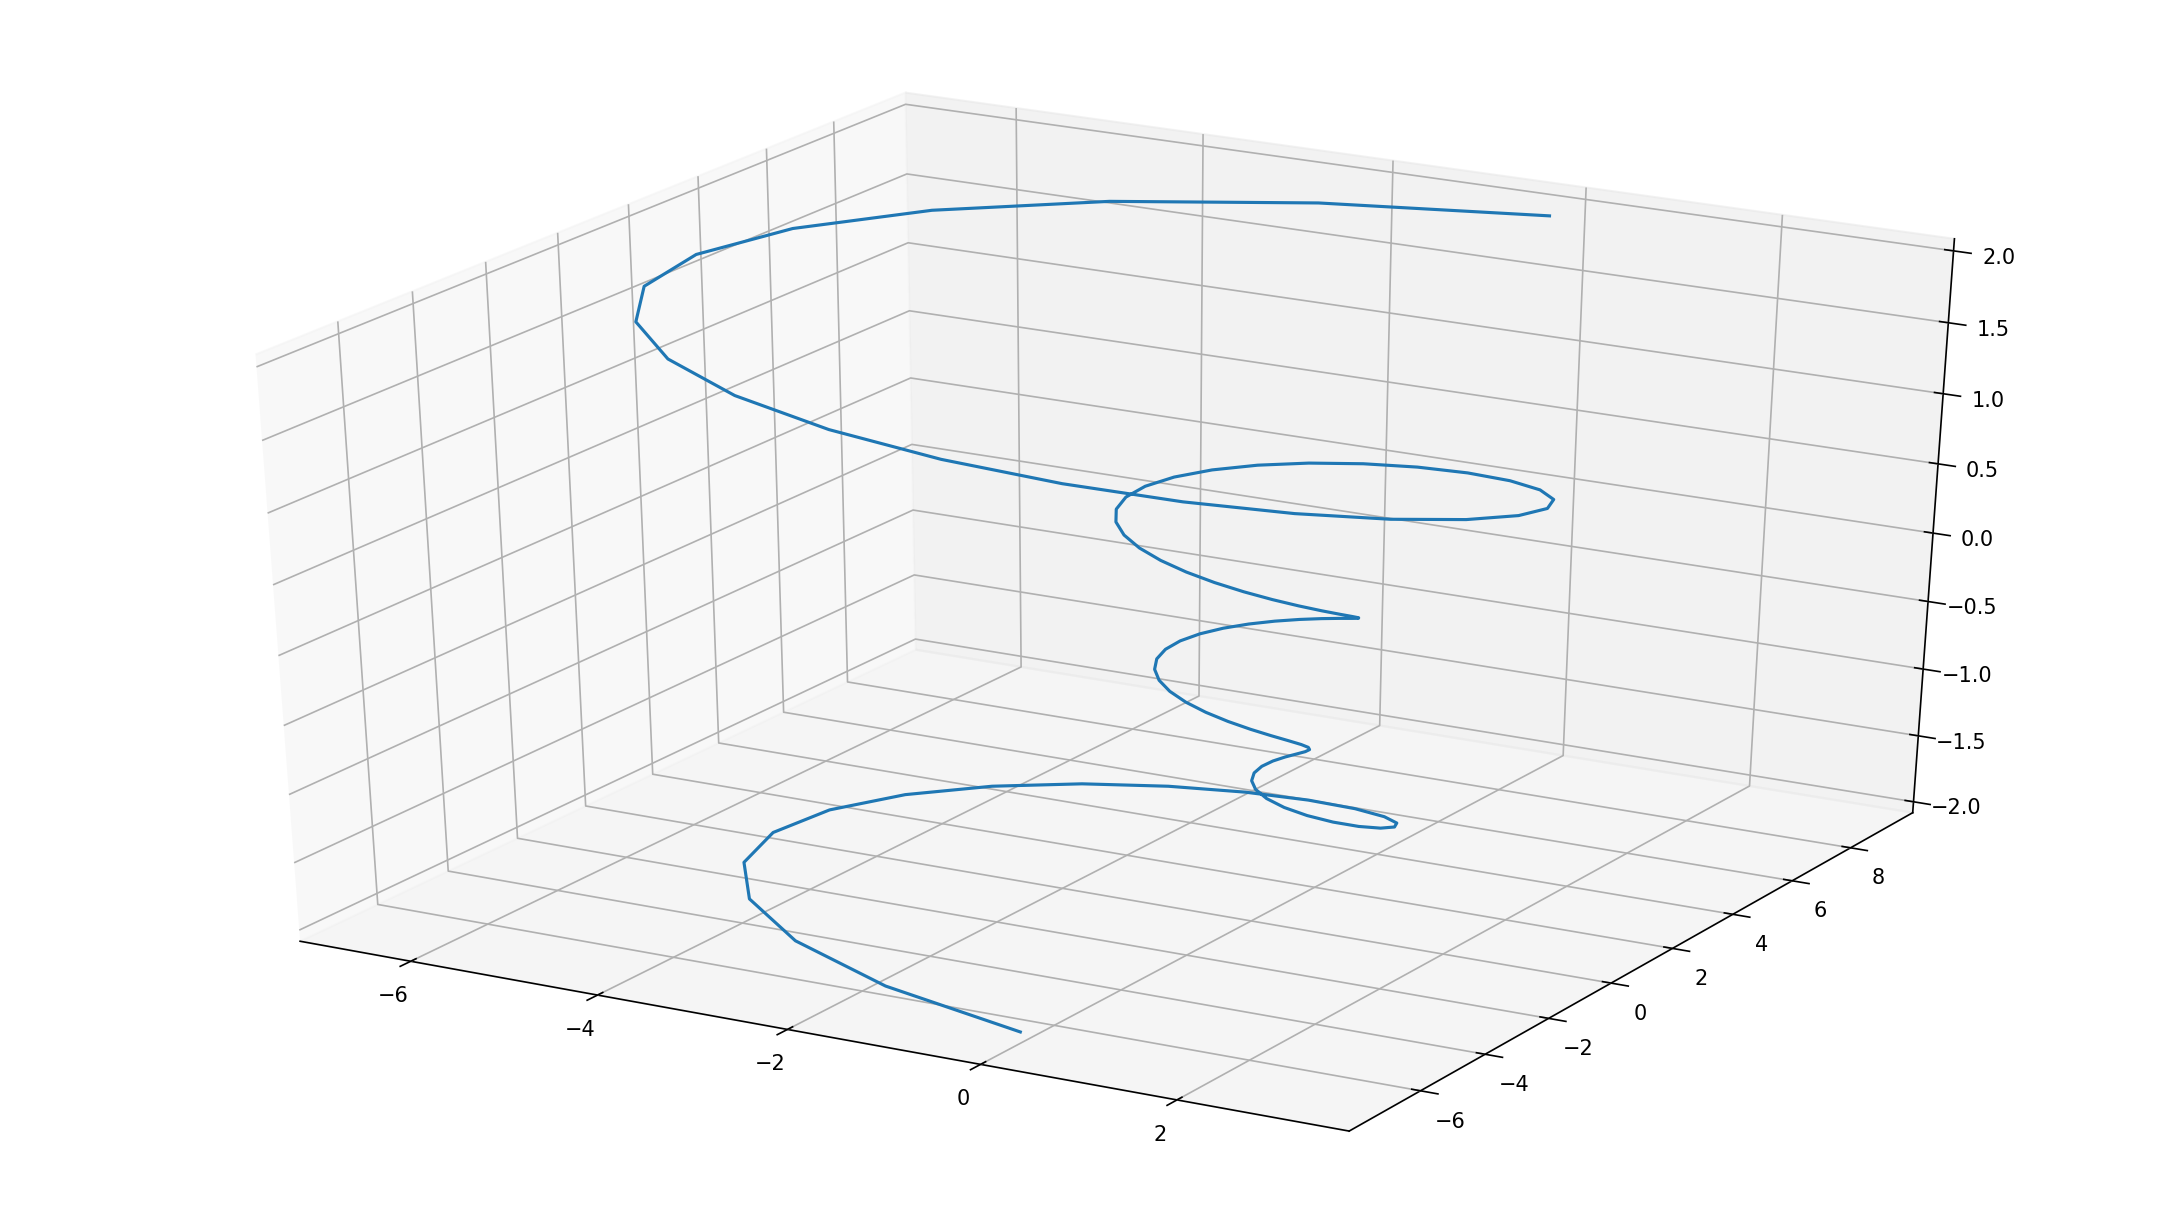
\includegraphics[width=\textwidth]{img/curve-1.png}
\caption{Térbeli ív szemléltetése.}
\label{fig:curve-1}
\end{figure}

A pontok által leírt ívet jeleníti meg egyetlen
töröttvonalként, de a \texttt{matplotlib} segítségével akár elhelyezhetjük rajta az adott diszkrét
pontokat is (\ref{fig:curve-2}. ábra):
\begin{python}
fig = plt.figure(figsize=(18.5, 10.5), dpi=150)
ax = fig.add_subplot(111, projection='3d')

theta = np.linspace(-4 * np.pi, 4 * np.pi, 100)
zline = np.linspace(-2, 2, 100)
r = z**3 + 1
xline = r * np.sin(theta)
yline = r * np.cos(theta)
ax.plot(xline, yline, zline)

zpoints = np.linspace(-2, 2, 100)
xpoints = r * np.sin(theta)
ypoints = r * np.cos(theta)
ax.scatter3D(xpoints, ypoints, zpoints, c=z, cmap="Reds")
plt.show()
\end{python}

\begin{figure}[h!]
\centering
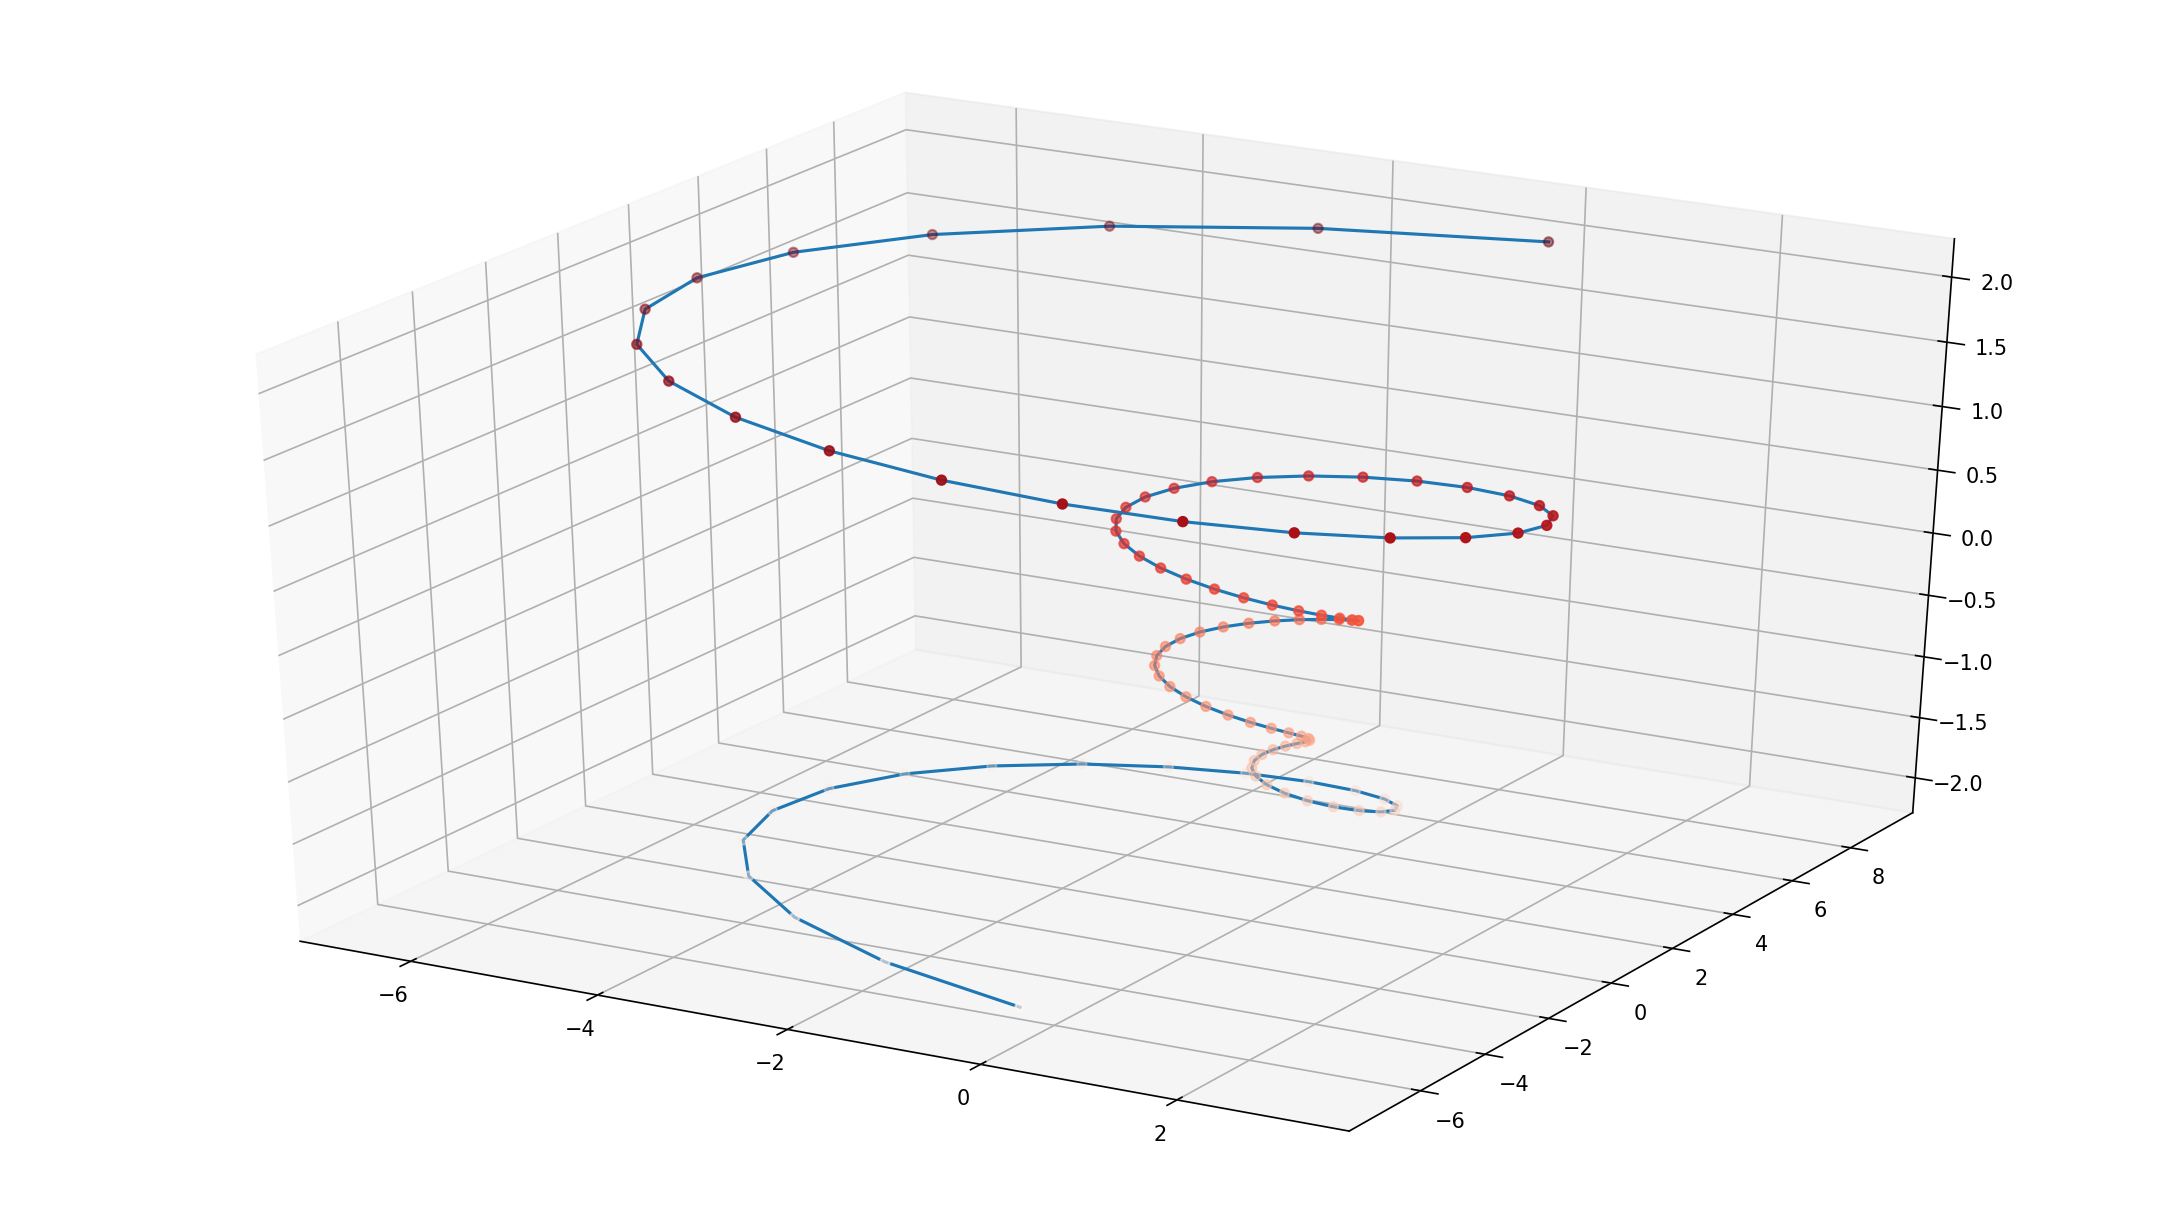
\includegraphics[width=\textwidth]{img/curve-2.png}
\caption{Térbeli ív szemléltetése diszkrét pontokkal együtt.}
\label{fig:curve-2}
\end{figure}
    
Megtehetjük azt is hogy cak a pontokat helyezzük el a 3D-s térben (\ref{fig:curve-3}. ábra):
\begin{python}
fig = plt.figure(figsize=(18.5, 10.5), dpi=150)
ax = fig.add_subplot(111, projection='3d')

theta = np.linspace(-4 * np.pi, 4 * np.pi, 100)
r = z**3 + 1
zpoints = np.linspace(-2, 2, 100)
xpoints = r * np.sin(theta)
ypoints = r * np.cos(theta)
ax.scatter3D(xpoints, ypoints, zpoints, c=z, cmap="hsv")
plt.show()
\end{python}

\begin{figure}[h!]
\centering
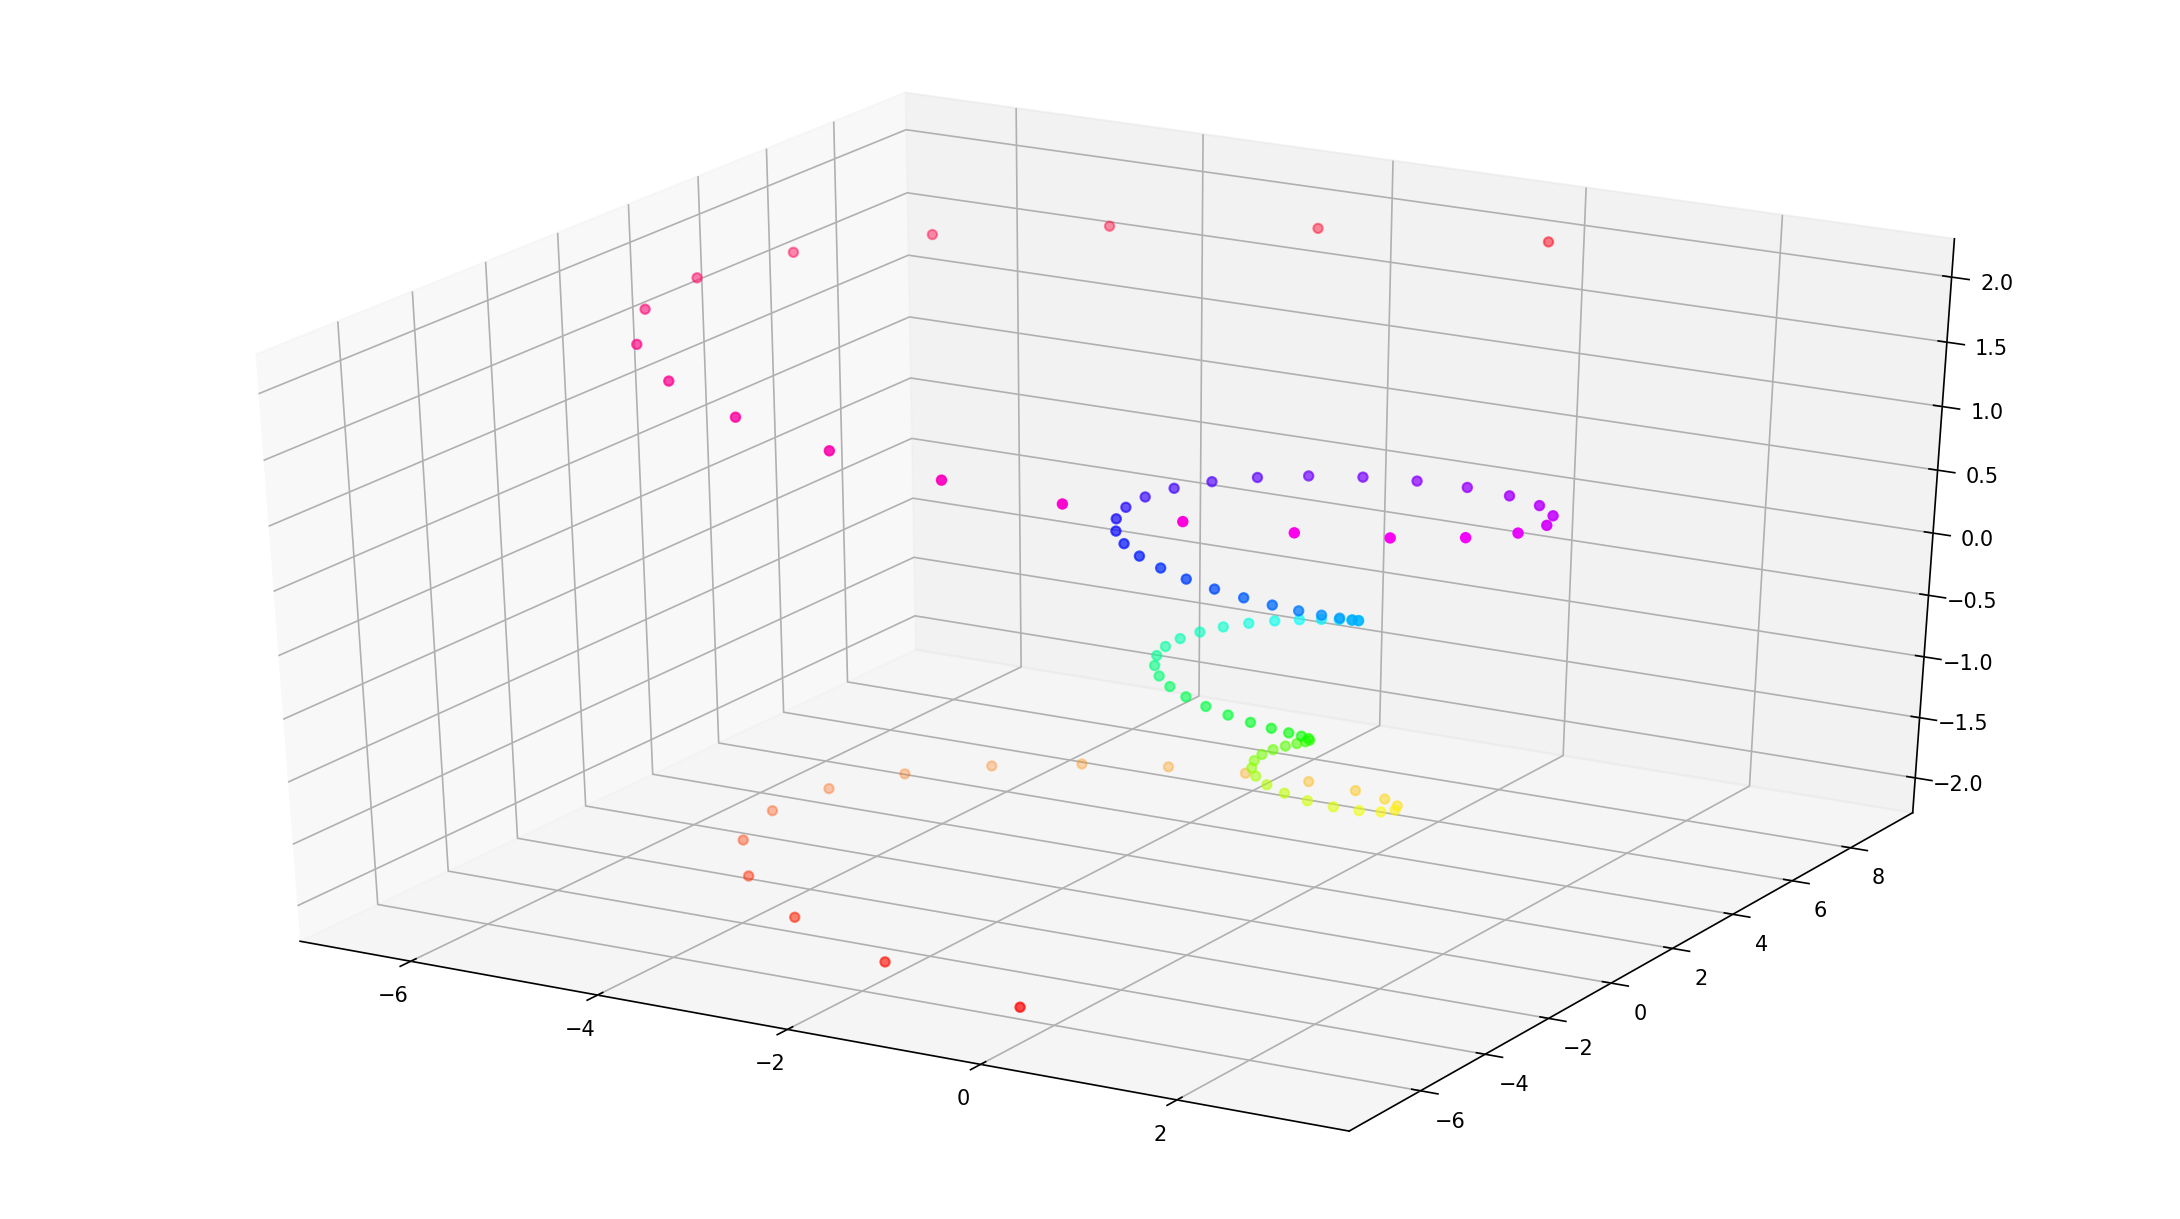
\includegraphics[width=\textwidth]{img/curve-3.png}
\caption{Térbeli pontok szemléltetése HSV színezéssel.}
\label{fig:curve-3}
\end{figure}
    
    Egy felületet megjeleníthetünk többféleképpen is a \textbf{wireframe}
segítségével egy háló szerűen, míg a \textbf{surface} használatával
egybefüggő felületként. A következő példában már a kapott térbeli felületi elforgatása is szerepel:
\begin{python}
def f(x, y):
    return np.sin(np.sqrt(x ** 2 + y ** 2))

x = np.linspace(-6, 6, 30)
y = np.linspace(-6, 6, 30)

X, Y = np.meshgrid(x, y)
Z = f(X, Y)

plt.figure(figsize=(18.5, 10.5), dpi=150)
ax = plt.axes(projection='3d')
ax.plot_surface(X, Y, Z, rstride=1, cstride=1,
                cmap='viridis', edgecolor='none')
ax.set_title('surface');
ax.view_init(60, 35)
\end{python}
Az így megjelenített felület \aref{fig:curve-4}. ábrán látható.

\begin{figure}[h!]
\centering
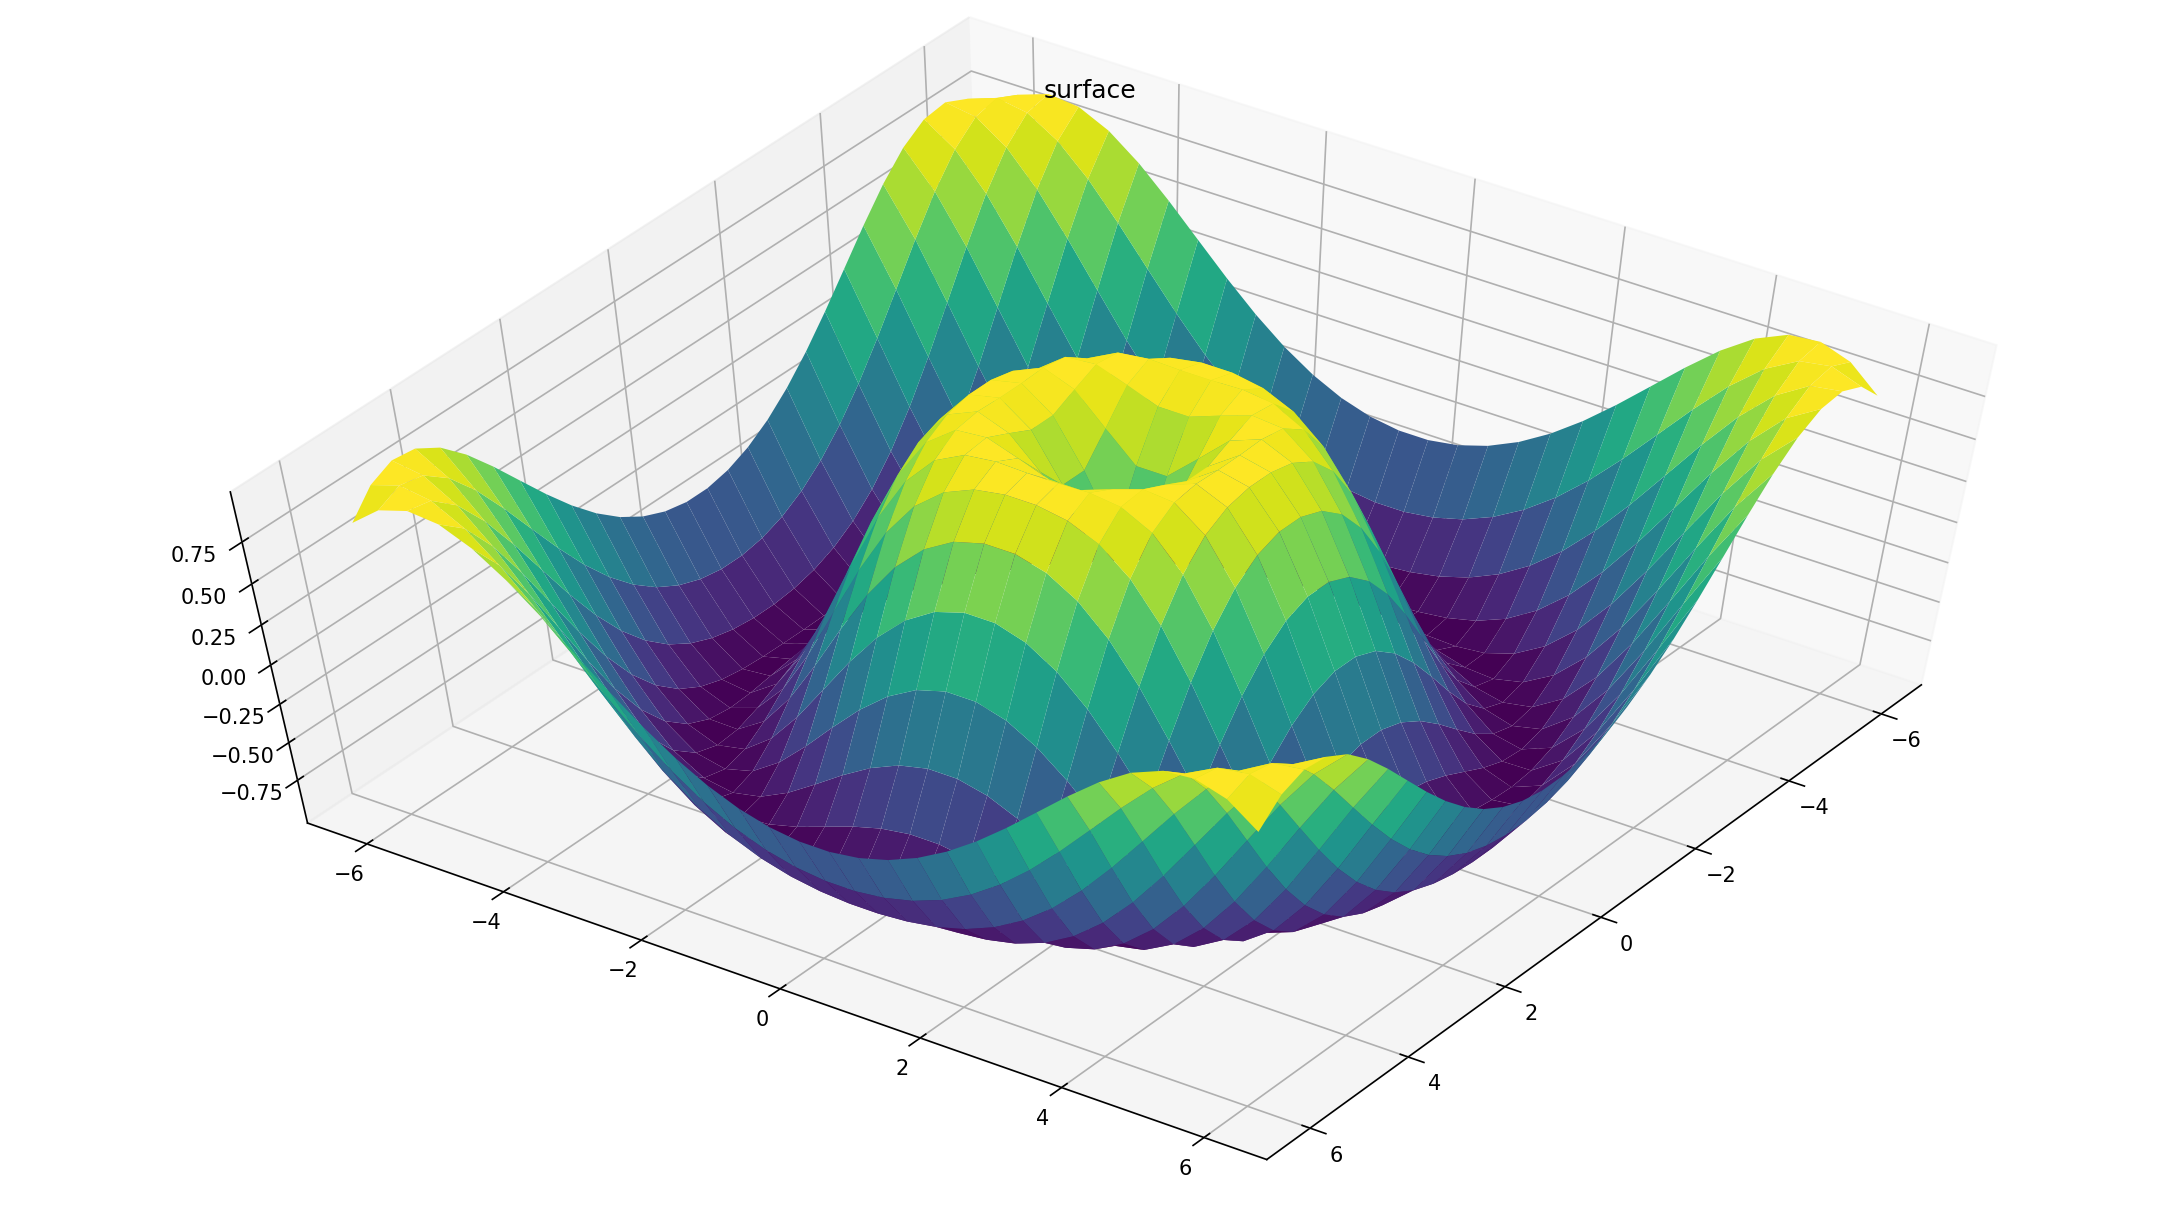
\includegraphics[width=\textwidth]{img/curve-4.png}
\caption{Térbeli felület megjelenítése.}
\label{fig:curve-4}
\end{figure}
    
    Sok más további lehetőséget is kínál a matplotlib, például megjeleníthetünk
3d-ben 2-ds adatokat, vagy készíthetünk 3d-s hisztogrammot több adattal,
de a fent említettek talán a legfontosabbak és legtöbbet használtak.

\Section{Interaktív widgetek Jupyter-ben}

Az interaktív plotokról csak említés szintjén esik szó a dolgozatban, hiszen ezek
készítését nem a Python, hanem a Jupyter notebook és a IPython kernel
teszi lehetővé. Az
\texttt{interact} segítségével tudunk interaktív dolgokat készíteni, például azért, hogy több adatra megnézhessük egy függvény képét. A következő
példában különböző hatvány függvényeket lehet megnézni, és a csúszka
segítségével lehet beállítani a hatvány kitevőt:
\begin{python}
from __future__ import print_function
from ipywidgets import interact, interactive, fixed, interact_manual
import ipywidgets as widgets
import matplotlib.pyplot as plt
import numpy as np
from ipywidgets import Button, Layout

def f(y):
    x = np.linspace(-100, 100, 100)
    plt.figure(figsize=(14, 7), dpi=150)
    plot = plt.plot(x, x**y)
    plt.show()

interact(f, y=widgets.IntSlider(min=1, max=30, step=1, value=0));
\end{python}
    
A minta számot is beállíthatjuk egy ilyen csúszkával és ezzel a pontosságot tudjuk szabályozni:
\begin{python}
def f(y):
    x = np.linspace(-10, 10, y)
    plt.figure(figsize=(14, 7), dpi=150)
    plot = plt.plot(x, x**2, 'o', color="green")
    plt.show()

interact(f, y=widgets.IntSlider(min=1, max=200, step=1, value=0));
\end{python}
Egy értékbeállítást láthatunk \aref{fig:interact-1}. ábrán.

\begin{figure}[h!]
\centering
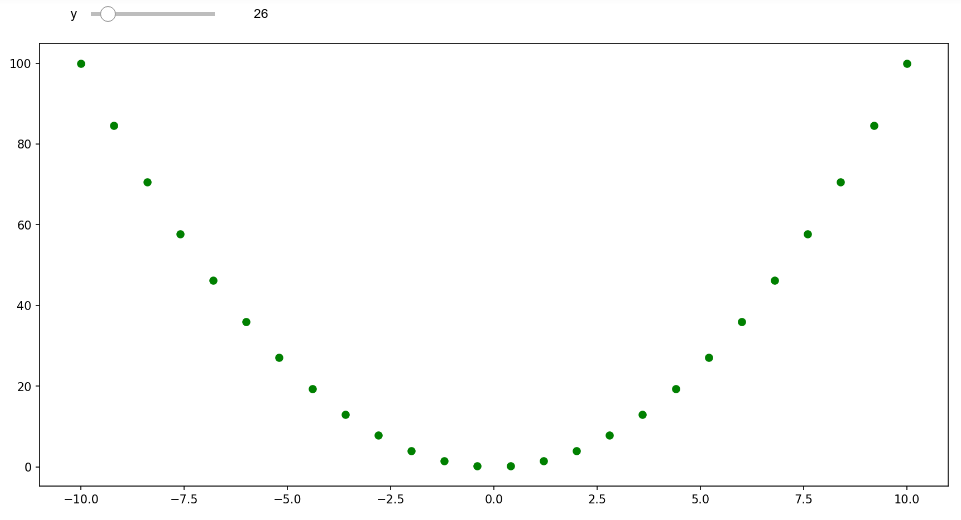
\includegraphics[width=\textwidth]{img/interact-1.png}
\caption{Csúszka használata.}
\label{fig:interact-1}
\end{figure}

    Az interaktivitásnak sok további formája van. Például
vannak még igaz/hamis értékekre állítható jelölőnégyzet  (\texttt{Checkbox}), szöveges
bevitelre alkalmas mező (\texttt{Text}), lenyíló
lista (\texttt{Dropdown}). Itt szerepel egy kis
példa egy szöveges mezőre mely összead két számot.
\begin{python}
def f(a, b):
    if a == "":
        x = 0
    else:
        x = float(a)
    if b == "":
        y = 0
    else:
        y = float(b)
    print(x + y)

interact(f, a="", b="");
\end{python}
    Fontos megjegyezni, hogy a beírt dolgok szövegként kerülnek átadásra, ezért szükség lehet azok számmá való konvertálására, ahogy az előbbi példában is látható.
    
    Megvalósításából fakadóan ezek az interaktív eszközök használhatóak 3D plotoknál, illetve más helyeken is.
Különösen hasznos lehet például térben ábrázolt felület forgatásánál. Ez az alábbi kódrészlettel valósítható meg.
\begin{python}
from mpl_toolkits.mplot3d import axes3d

def f(x, y):
    return np.sin(np.sqrt(x ** 2 + y ** 2))

def g(angle1, angle2):
    x = np.linspace(-6, 6, 30)
    y = np.linspace(-6, 6, 30)

    X, Y = np.meshgrid(x, y)
    Z = f(X, Y)

    plt.figure(figsize=(14, 7), dpi=150)
    ax = plt.axes(projection='3d')
    ax.plot_surface(X, Y, Z, rstride=1, cstride=1,
                    cmap='viridis', edgecolor='none')
    ax.set_title('surface');
    ax.view_init(angle1, angle2)
    
interact(g,
    angle1=widgets.IntSlider(min=0, max=360, step=1, value=0,
        layout=Layout(width="600px")),
    angle2=widgets.IntSlider(min=0, max=360, step=1, value=0,
        layout=Layout(width="600px")));
\end{python}

\Chapter{Összefoglalás}



\clearpage

\addcontentsline{toc}{chapter}{Irodalomjegyzék}
\bibliographystyle{plain}
\bibliography{dolgozat.bib}

\newpage

\pagestyle{empty}

\noindent \textbf{\Large A CD melléklet tartalma}

\vskip 1cm

\noindent A CD-n a következő mellékletek szerepelnek.
\begin{itemize}
\item A dolgozatot egy \texttt{dolgozat.pdf} fájl formájában,
\item A dolgozat \LaTeX\ forráskódja a \texttt{szakdolgozat} jegyzékben.
\item A dolgozathoz készített Jupyter munkafüzetek a \texttt{notebooks} jegyzékben.
\end{itemize}

\vskip 17cm

\emph{A cikkben/előadásban/tanulmányban ismertetett kutató munka az
EFOP-3.6.1-16-2016-00011 jelű „Fiatalodó és Megújuló Egyetem –
Innovatív Tudásváros – a Miskolci Egyetem intelligens szakosodást
szolgáló intézményi fejlesztése” projekt részeként – a
Széchenyi 2020 keretében – az Európai Unió támogatásával, az
Európai Szociális Alap társfinanszírozásával valósul meg"}


\end{document}
